% !TEX encoding = UTF-8
%Koma article
\documentclass[fontsize=12pt,paper=letter,twoside]{scrartcl}
\usepackage{float}
\usepackage{listings}

%Standard Pre-amble
\usepackage[top=4cm,bottom=4cm,left=3cm,right=3cm,asymmetric]{geometry}
%\geometry{landscape}                % Activate for for rotated page geometry
%\usepackage[parfill]{parskip}    % Begin paragraphs with an empty line rather than an indent
\usepackage[table,xcdraw]{xcolor}
\usepackage{graphicx}

\usepackage{amsmath}
\usepackage{amssymb}
\usepackage{epstopdf}
\DeclareGraphicsRule{.tif}{png}{.png}{`convert #1 `dirname #1`/`basename #1 .tif`.png}
% Listings needs package courier
\usepackage{listings} % Needs 
\usepackage{courier}

\usepackage[framemethod=TikZ]{mdframed}
\usepackage{url}

\usepackage{sty/bsymb} %% Event-B symbols
\usepackage{sty/eventB} %% REQ and ENV
\usepackage{sty/calculation}

%Maths
\usepackage{amssymb,amsmath}
\def\Fl{\mathbb{F}}
\def\Rl{\mathbb{R}}
\def\Nl{\mathbb{N}}
\def\Bl{\mathbb{B}}
\def\St{\mathbb{S}}
\newcommand{\ovr}{\upharpoonright}
\newcommand{\var}[1]{\textit{#1}}
%Useful definitions
\newcommand{\mv}[1]{\textit{m\_#1}}
\newcommand{\cv}[1]{\textit{c\_#1}}
\newcommand{\degree}[1]{^{\circ}\mathrm{#1}}
%\newcommand{\comment}[1]{{\footnotesize \quad\texttt{--}\textrm{#1}}}
\newcommand{\im}[1]{i\texttt{-\!#1}}

\usepackage[headsepline]{scrpage2}
\pagestyle{scrheadings}
\ihead[]{\small EECS4312 Report1}
\ohead[]{\small \thepage}
\cfoot[]{}
\ofoot[]{}


%%%%PVS environment%%%%%%%%%%%%%%%%%%%
\lstnewenvironment{pvs}[1][]
    {\lstset{#1,captionpos=b,language=pvs,
    mathescape=true,
    basicstyle=\small\ttfamily,
    numbers=none,
    frame=single,
    % numberstyle=\tiny\color{gray},
    % backgroundcolor=\color{lightgray},
    firstnumber=auto
    }}
    {}
 %%%%%%%%%%%%%%%%%%%%%%%%%%%%%%%%
 
%%%%Verbatim environment%%%%%%%%%%%%%%%%%%%
\lstnewenvironment{code}[1][]
    {\lstset{#1,captionpos=b,
    mathescape=true,
    basicstyle=\small\ttfamily,
    numbers=none,
    frame=single,
    % numberstyle=\tiny\color{gray},
    % backgroundcolor=\color{lightgray},
    firstnumber=auto
    }}
    {}

% \newenvironment{boxed}[1]
%    {\begin{center}
%    #1\\[1ex]
%    \begin{tabular}{|p{0.9\textwidth}|}
%    \hline\\
%    }
%    { 
%    \\\\\hline
%    \end{tabular} 
%    \end{center}
%    }
 %%%%%%%%%%%%%%%%%%%%%%%%%%%%%%%%
 
 %Text in a box
\newenvironment{textbox}
    {\begin{center}
    \begin{tabular}{|p{0.9\textwidth}|}
    \hline\\
    }
    { 
    \\\\\hline
    \end{tabular} 
    \end{center}
    }

\usepackage{hyperref}

%Highlight \hl{}
\usepackage{soul}

\usepackage{enumitem}
\newlist{mylist}{itemize}{1}
\setlist[mylist]{label=\textbullet,leftmargin=1cm,nosep}

\usepackage{multirow}

% Reduce space between figure and caption
%\usepackage{caption}
%\captionsetup[table]{font=small,skip=0pt}     %% Adjust here
%or equivalently 
\usepackage[font=small,skip=4pt]{caption}
%Useful definitions
%\newcommand{\mv}[1]{\textit{m\_#1}}
%\newcommand{\cv}[1]{\textit{c\_#1}}
%\newcommand{\degree}[1]{^{\circ}\mathrm{#1}}
%\newcommand{\comment}[1]{{\footnotesize \quad\texttt{--}\textrm{#1}}}

% Set the header
\ihead[]{\small Gradapps}


%%%%%%%%%%%%Enter your names here%%%%%%%%
\author{\textbf{Edward Vaisman}
\and \textbf{Sadman Sakib Hasan}
}
%%%%%%%%%%%%%%%%%%%%%%%%%%%%%%%%

\date{\today} % Display a given date or no date

\begin{document}
\title{Grad Apps 2.0 \\ Administrator User Manual}
\maketitle

\newpage

%%%%%%%%%%%%%%%%%%%%%%%%%%%%%%%
\tableofcontents

\newpage


%%%%Rest of your document goes here%%%%%%%%%%%%%%%%%%%

\clearpage
\section{Logging In}

To access the gradapps portal you'll first need to be authenticated into the system. To begin simply click on the ``Sign In" button on the welcome page.

\begin{figure}[!htb]
\begin{center}

\includegraphics[width=.99\textwidth]{images/welcome.png}
\end{center}
\caption{Welcome Page}
\label{fig:welcome}
\end{figure}

\bigskip

You will then be redirected to the login page. Input your username, password and click on the ``Login" button. If you are successfully authenticated you will be redirected to the role selection page.

\begin{figure}[!htb]
\begin{center}
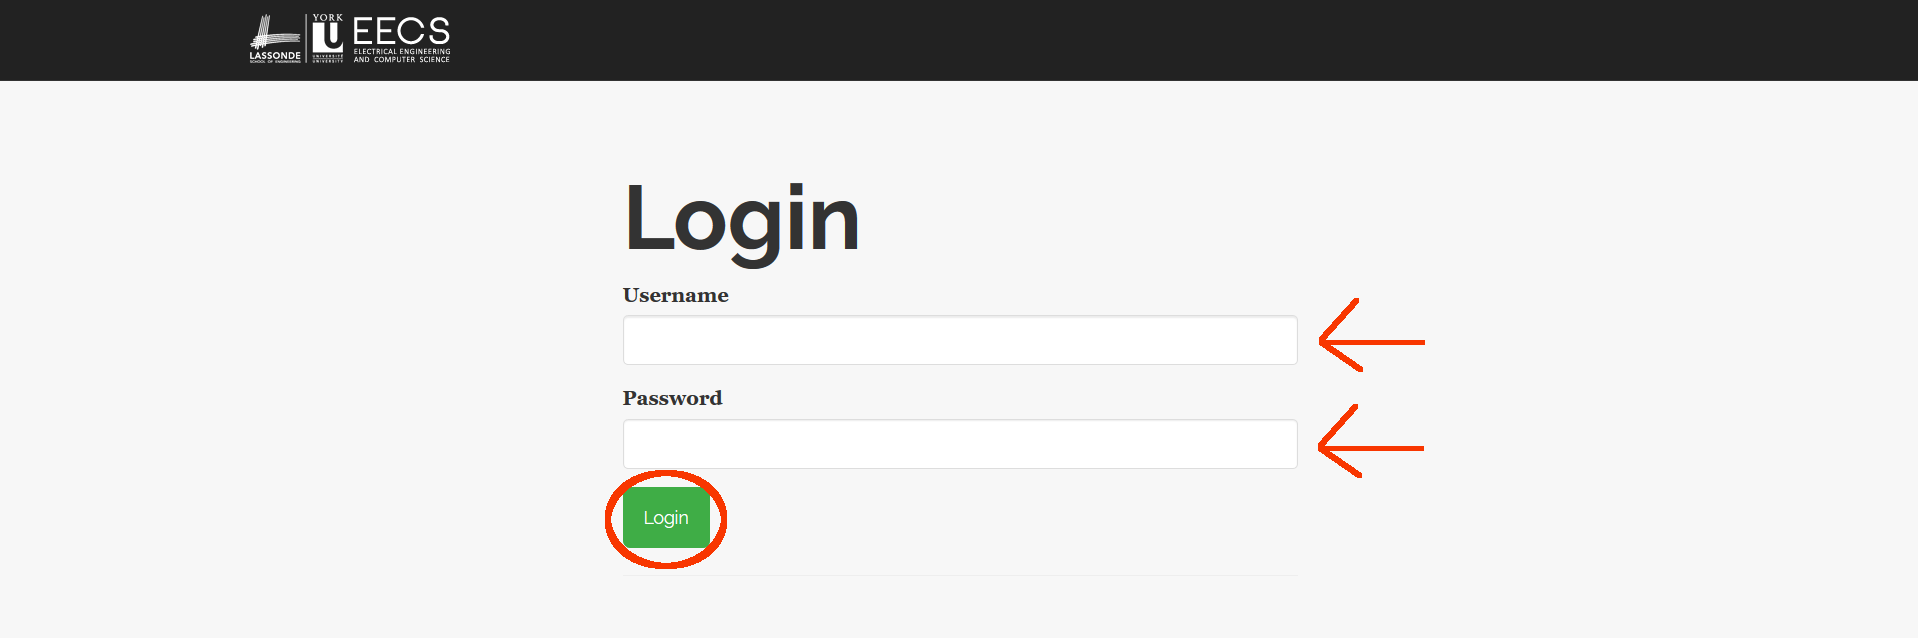
\includegraphics[width=.99\textwidth]{images/login.png}
\end{center}
\caption{Login Page}
\label{fig:login}
\end{figure}
\noindent \textbf{Note:} If the credentials you have provided are invalid you will be greeted with an error message.

\clearpage

\section{Selecting a Role}
The subsections below describe the methods for selecting the a role.

\subsection{Role Selection Page}
From the role selection page click on the ``Continue as an Admin" button to be redirected to the committee member portal.

\begin{figure}[!htb]
\begin{center}
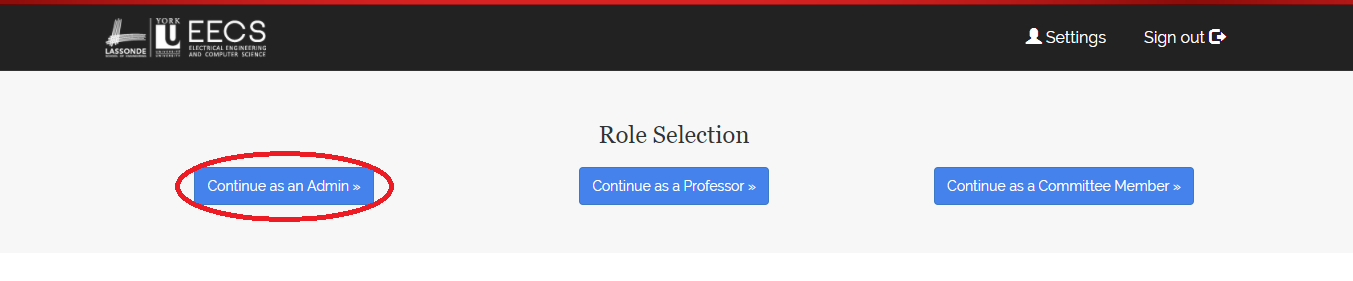
\includegraphics[width=.99\textwidth]{images/auth.png}
\end{center}
\caption{Role Selection Page}
\label{fig:role_selection1}
\end{figure}

\noindent \textbf{Note:} To access the administrator/committee/professor portal you must be granted access from an administrator.

\subsection{Navigation Bar}
If you have selected another role and wish to switch roles you will be presented with an option on the navigation bar. Click on the dropdown menu that displays your current role and click on your desired role.
\begin{figure}[!htb]
\begin{center}
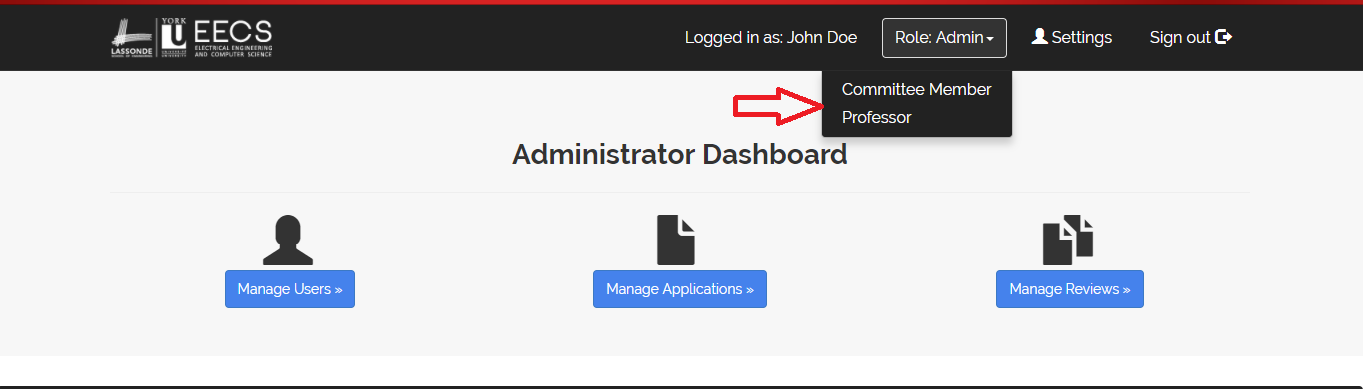
\includegraphics[width=.9\textwidth]{images/role-selection2.png}
\end{center}
\caption{Switch Roles}
\label{fig:role_selection2}
\end{figure}

\noindent \textbf{Note:} To access the administrator/committee/professor portal you must be granted access from an administrator.

\section{Administrator Dashboard}

After logging in and selecting the \emph{Admin} role you will have access to the administrator dashboard. From the dashboard you can perform the following:
\begin{itemize}
\item Manage Users (Refer to section: \ref{m_user})
\begin{itemize}
\item Adding a new user
\item Remove an existing user
\item Assign a new role to an user
\item Removing a role from an user
\item Updating user information such as:
\begin{itemize}
\item Username
\item Password
\item Last Name
\item First Name
\item Email Address
\item Field(s) of Specialization
\end{itemize}
\item Deleting unwanted filter presets
\end{itemize}
\item Manage Applications (Refer to section: \ref{m_appls})
\begin{itemize}
\item Creating a new application
\item Deleting an existing application
\item Apply filtering on existing application(s)
\item Save presets on most used filter(s)
\item Export all or a set of application(s) to CSV
\item View application PDF file
\end{itemize}
\item Manage Reviews (Refer to section: \ref{m_reviews})
\begin{itemize}
\item Assign at most one reviewer for visa applicants
\item Assign at most two reviewer(s) for domestic applicants
\item Unassign reviews from an application
\item Dismiss submitted review from an application
\item View application PDF file
\end{itemize}
\end{itemize} 

\smallskip
\noindent More on each of the three management portals in the following sections.

\clearpage
\begin{figure}[!htb]
\begin{center}
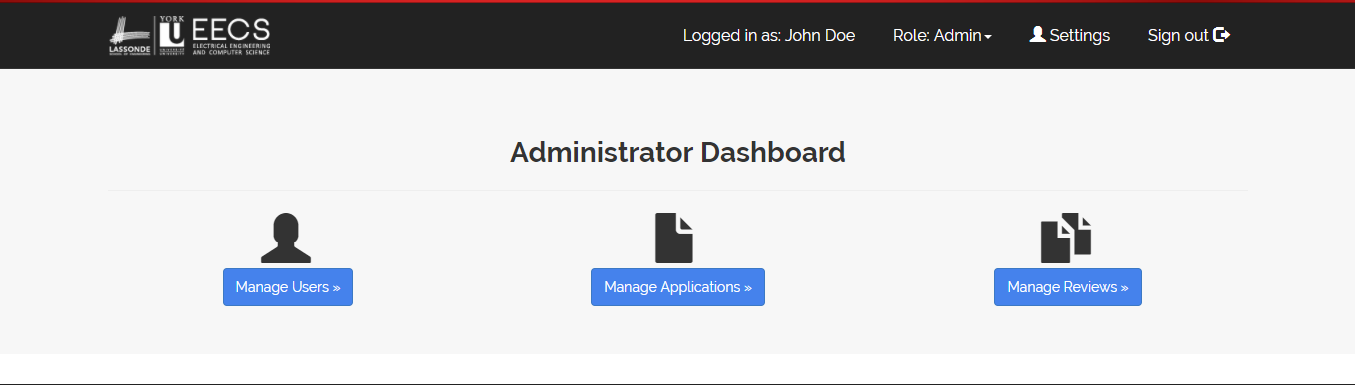
\includegraphics[width=.99\textwidth]{images/admin_dash.png}
\end{center}
\caption{Administrator Dashboard}
\label{fig:admin_dash}
\end{figure}

\smallskip
\noindent \textbf{Note:} Each of the management portal has a \emph{Go back to dashboard} link which upon clicking will bring back to the default dashboard.


%%%%%%%%% MANAGE USER %%%%%%%%%%
\newpage
\clearpage
\section{Manage Users} \label{m_user}
This section describes how you would add/remove a user, assign/unassign roles from a user and update user related information. To begin, from the administrator dashboard, click on \emph{Manage Users}.

\begin{figure}[!htb]
\begin{center}
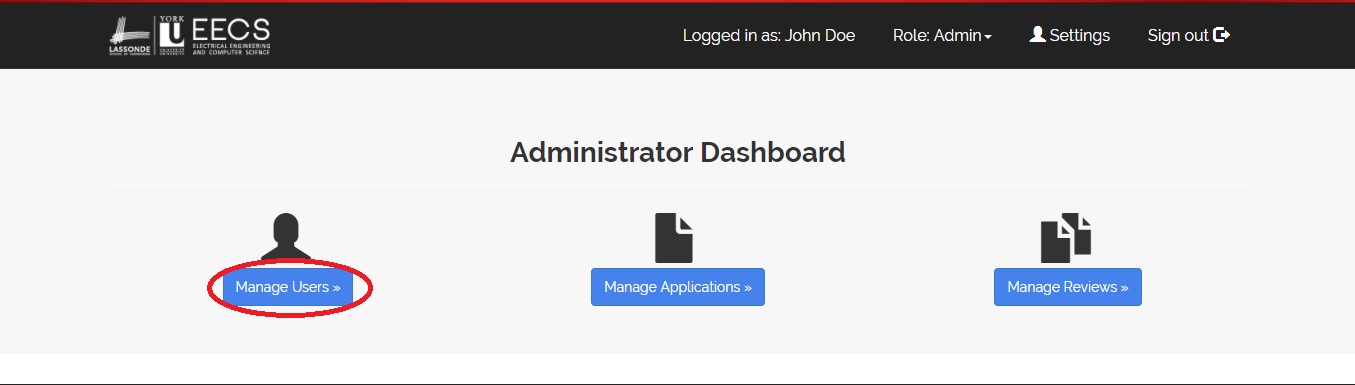
\includegraphics[width=.99\textwidth]{images/mu/manage_user.png}
\end{center}
\caption{Click to Manage Users}
\label{fig:manage_user}
\end{figure}

\subsection{Adding a user}
Once in the managing user portal, you can add a new user to the system. Adding a new user to the system requires you to give them a username (EECS username), generate a random password or make a password for the user, fill in basic user information (such as Last Name, First Name, Email Address, Field(s) of Specialization) and assign them a role. The following fields are required when creating a new user:
\begin{itemize}
\item Username
\item Password
\item Last Name
\item First Name
\item Email
\item Role(s)
\end{itemize}

\smallskip
\noindent \textbf{Note:} Username for a user is unique and hence trying to create a user with an existing username will not allow the new user to be created.

\begin{figure}[!htb]
\begin{center}
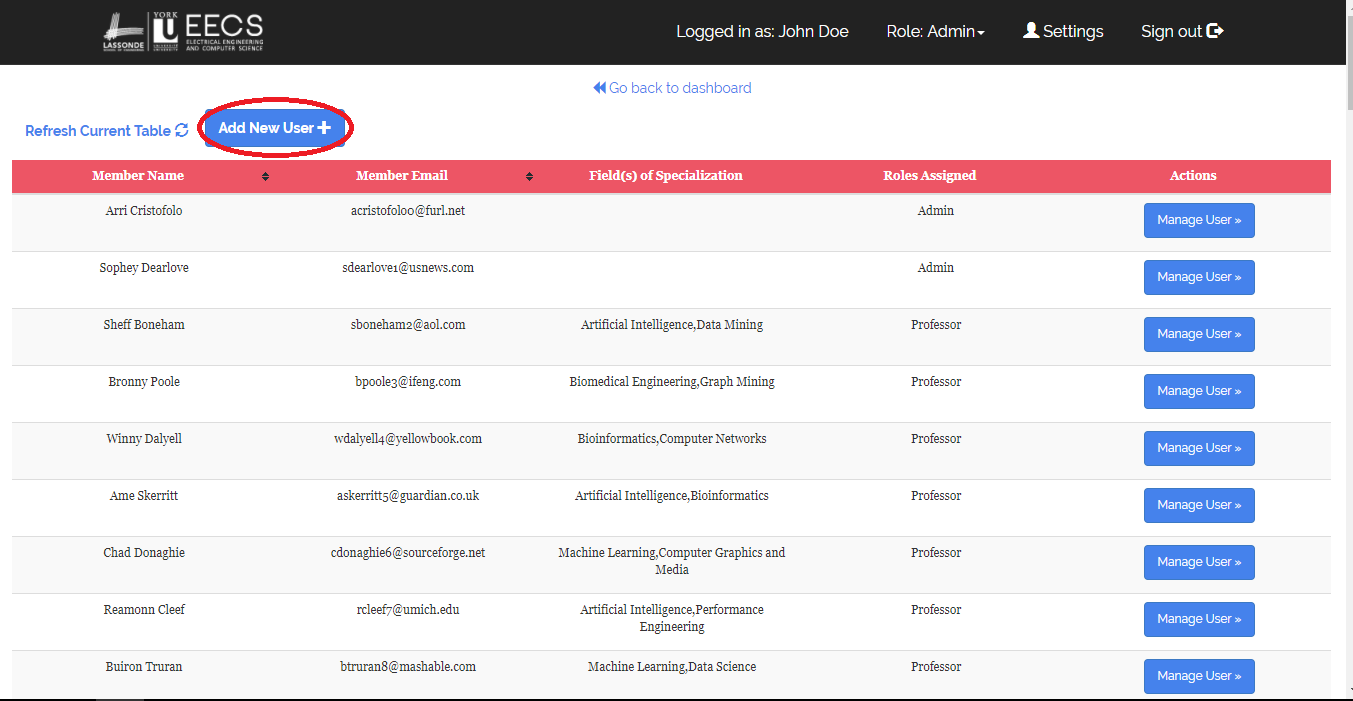
\includegraphics[width=.99\textwidth]{images/mu/new_user_click.png}
\end{center}
\caption{Click to create a user}
\label{fig:new_user_click}
\end{figure}

\begin{figure}[!htb]
\begin{center}
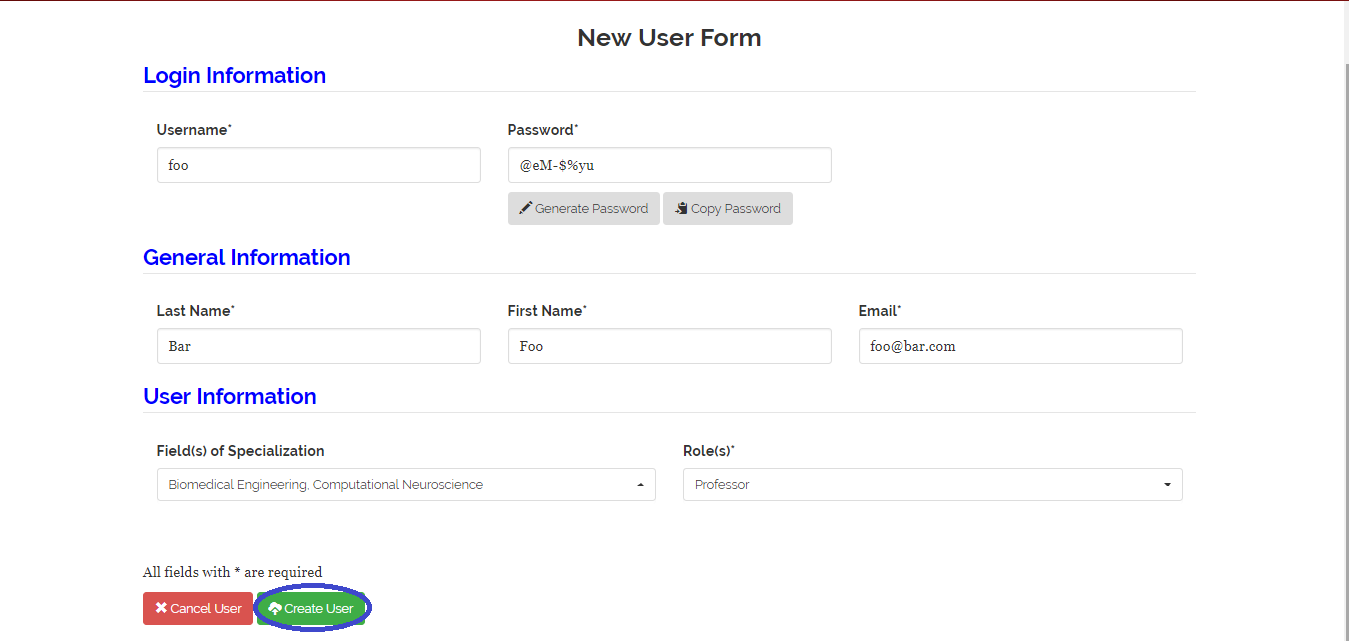
\includegraphics[width=.99\textwidth]{images/mu/fill_in_user.png}
\end{center}
\caption{Filling in user information}
\label{fig:fill_in_user}
\end{figure}

\clearpage
\subsection{Edit existing user}
Once in the managing user portal, you can edit an existing user. Editing includes updating user information, assigning/unassigning roles or removing the user completely from the system.

\begin{figure}[!htb]
\begin{center}
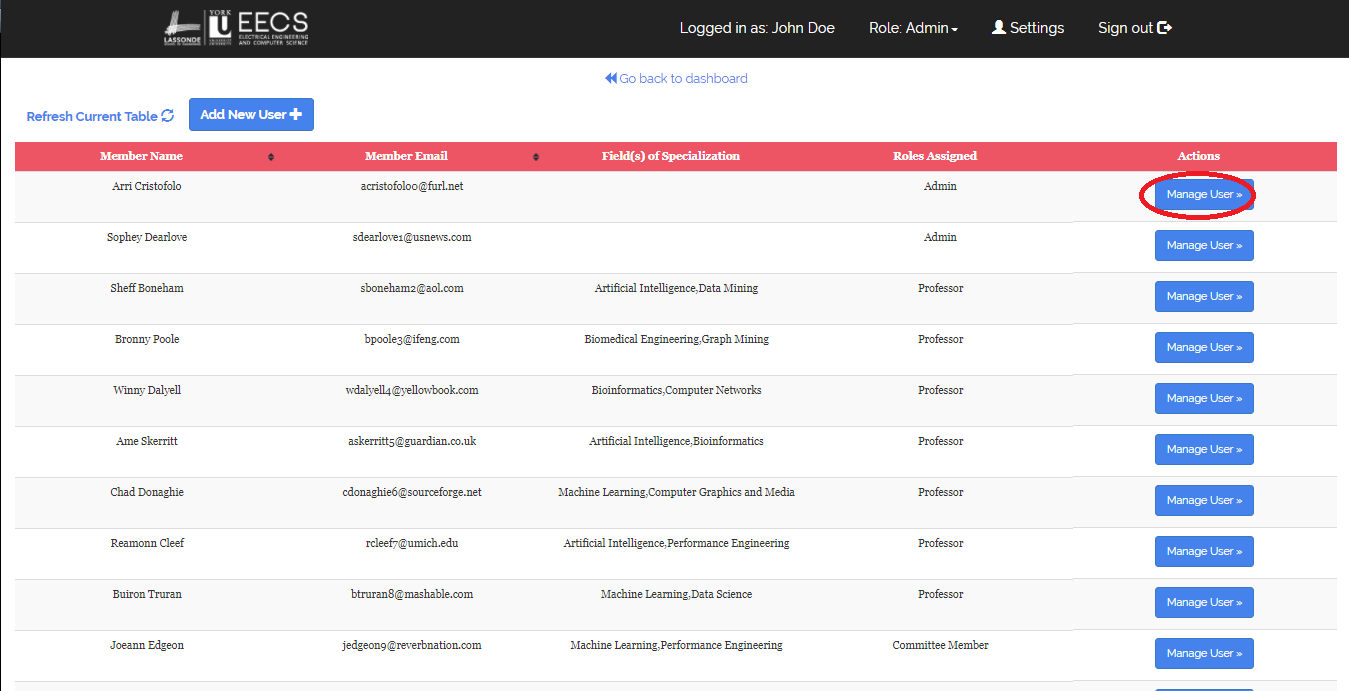
\includegraphics[width=.99\textwidth]{images/mu/edit_user.png}
\end{center}
\caption{Click to edit an user}
\label{fig:edit_user}
\end{figure}

\smallskip
\noindent \textbf{Note:} An administrator cannot edit their own user settings from the manage user portal. Another administrator has to edit it for them. However, they can update their own personal settings like any other user from the \emph{Settings} menu in the navbar. 

\begin{figure}[!htb]
\begin{center}
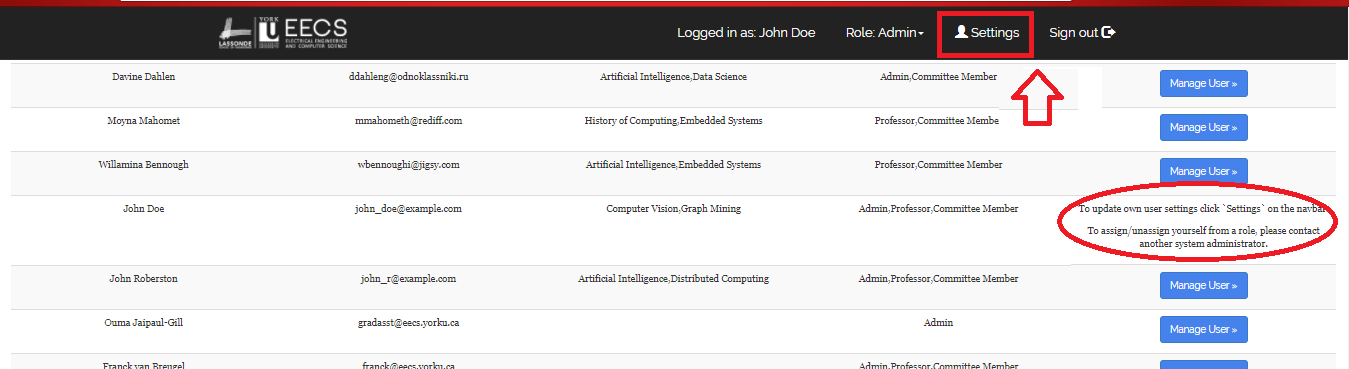
\includegraphics[width=.99\textwidth]{images/mu/edit_own_user.png}
\end{center}
\caption{Editing own user settings}
\label{fig:edit_own_user}
\end{figure}

\clearpage
\subsubsection{Remove an user}
To remove an existing user from the system, click on the \emph{Manage User} button as shown above for the corresponding user. Then click on the trash can button at the bottom of the page as shown.

\smallskip
\noindent \textbf{Note:} As an administrator you can only remove other users. You cannot remove yourself from the system. Another administrator has to remove you in that case.

\begin{figure}[!htb]
\begin{center}
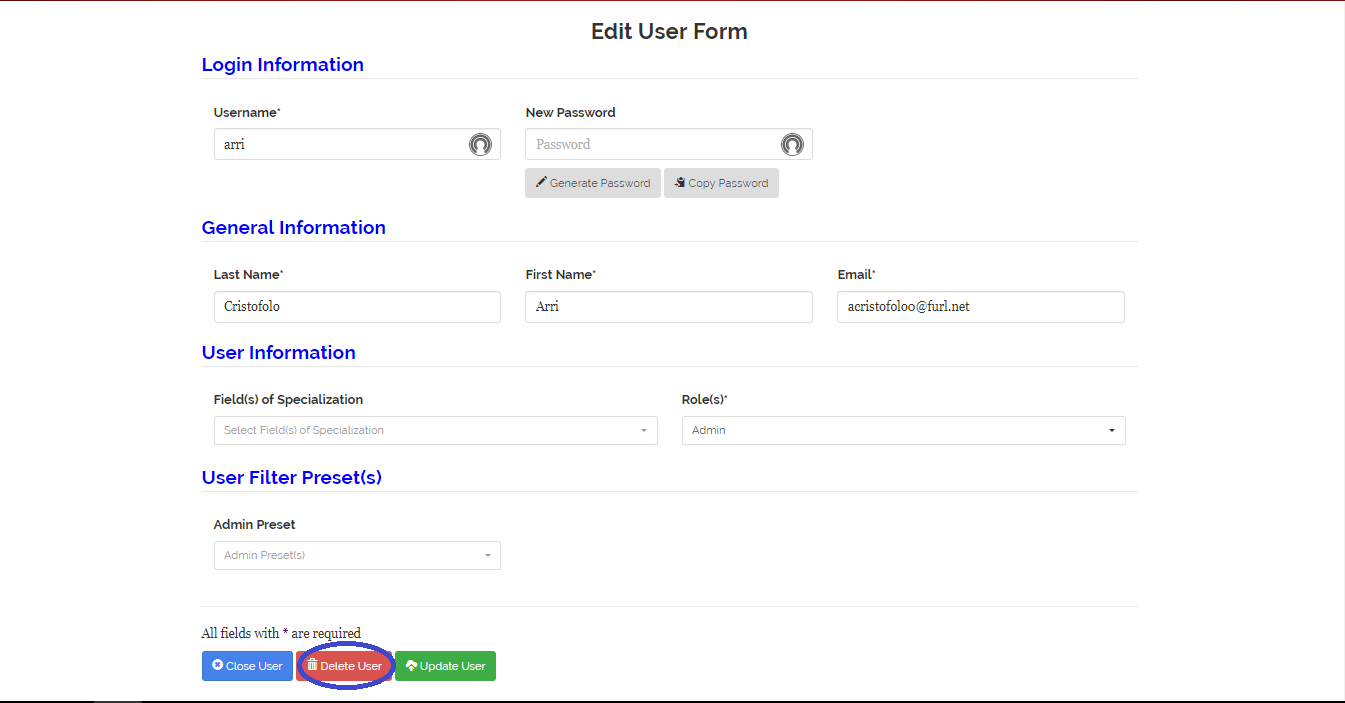
\includegraphics[width=.99\textwidth]{images/mu/remove_user.png}
\end{center}
\caption{Removing an user}
\label{fig:remove_user}
\end{figure}

\clearpage
\subsubsection{Assign/Unassign roles}
To assign or unassign a role from an existing user from the system, click on the \emph{Manage User} button as shown above for the corresponding user. Then select or de-select the role you want to assign or unassign for the user.

\smallskip
\noindent \textbf{Note:} A user must have at least one role assigned to them at all times.

\begin{figure}[!htb]
\begin{center}
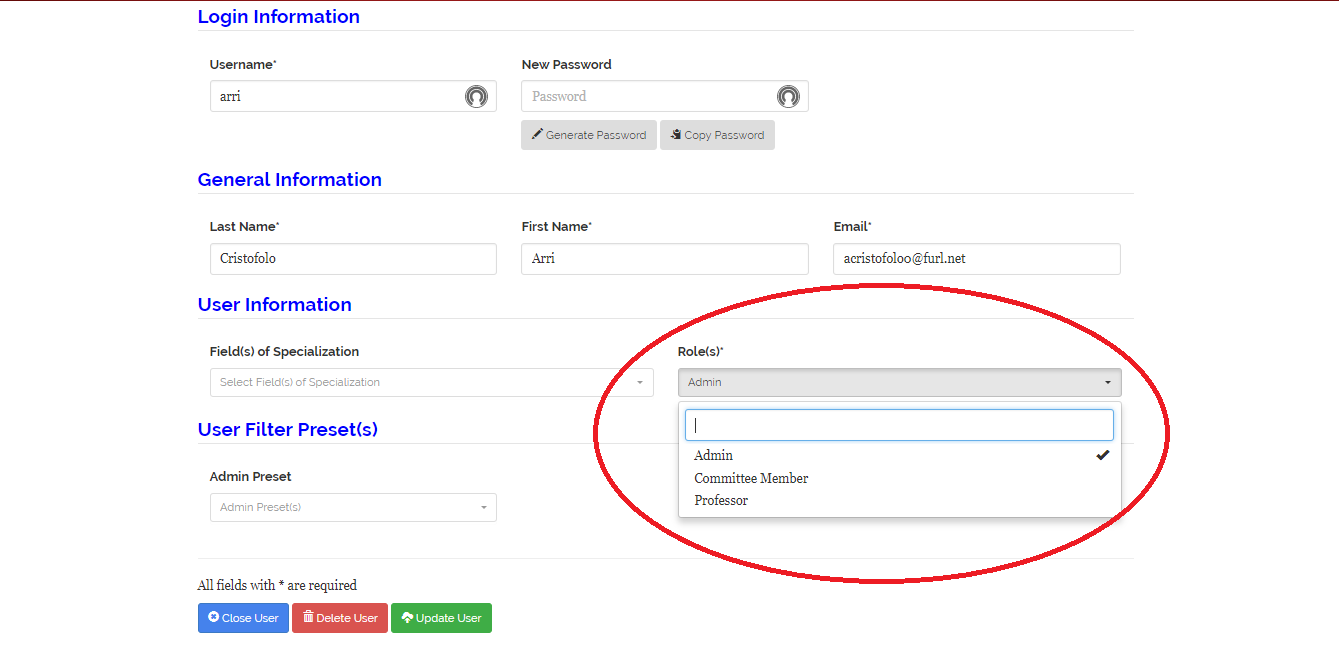
\includegraphics[width=.99\textwidth]{images/mu/edit_roles.png}
\end{center}
\caption{Assign/Unassign roles}
\label{fig:edit_roles}
\end{figure}

\clearpage
\subsubsection{Update User Information}
As an administrator you can update user information. To update user information for an existing user, click on the \emph{Manage user} button as shown above for the corresponding user. Then click on the upload button at the bottom of the page as shown. The following fields are required when updating a user information:
\begin{itemize}
\item Username
\item Last Name
\item First Name
\item Email
\item Role(s)
\end{itemize}

\smallskip
\noindent \textbf{Note:} All required fields are needed to be filled when editing an user.

\begin{figure}[!htb]
\begin{center}
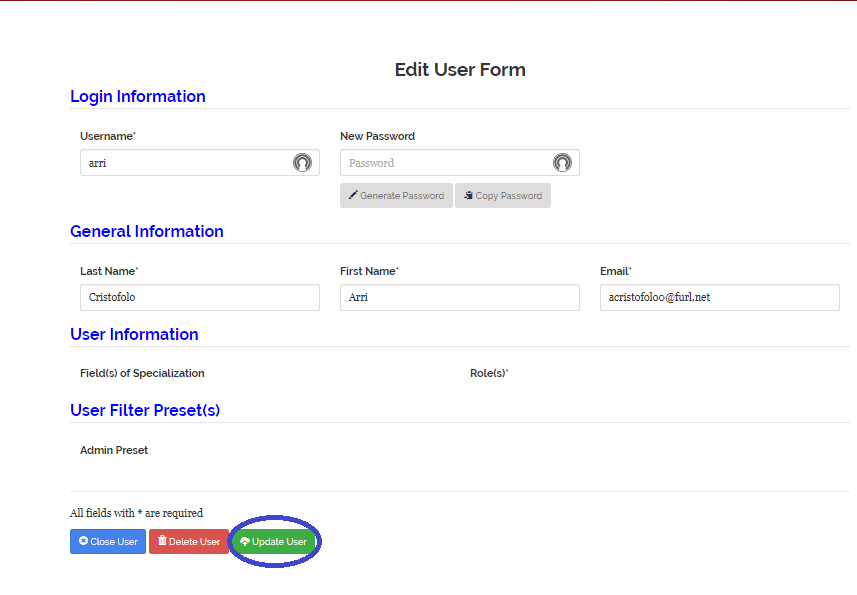
\includegraphics[width=.9\textwidth]{images/mu/update_user.png}
\end{center}
\caption{Updating an user}
\label{fig:update_user}
\end{figure}

\clearpage
\subsubsection{Remove Unwanted Filter Presets}
As an administrator you can remove unwanted filter presets for a particular user. To remove such presets for an existing user, click on the \emph{Manage user} button as shown above for the corresponding user. Then simply unchecking the preset from the dropdown will permanently remove the preset for the user.

\begin{figure}[!htb]
\begin{center}
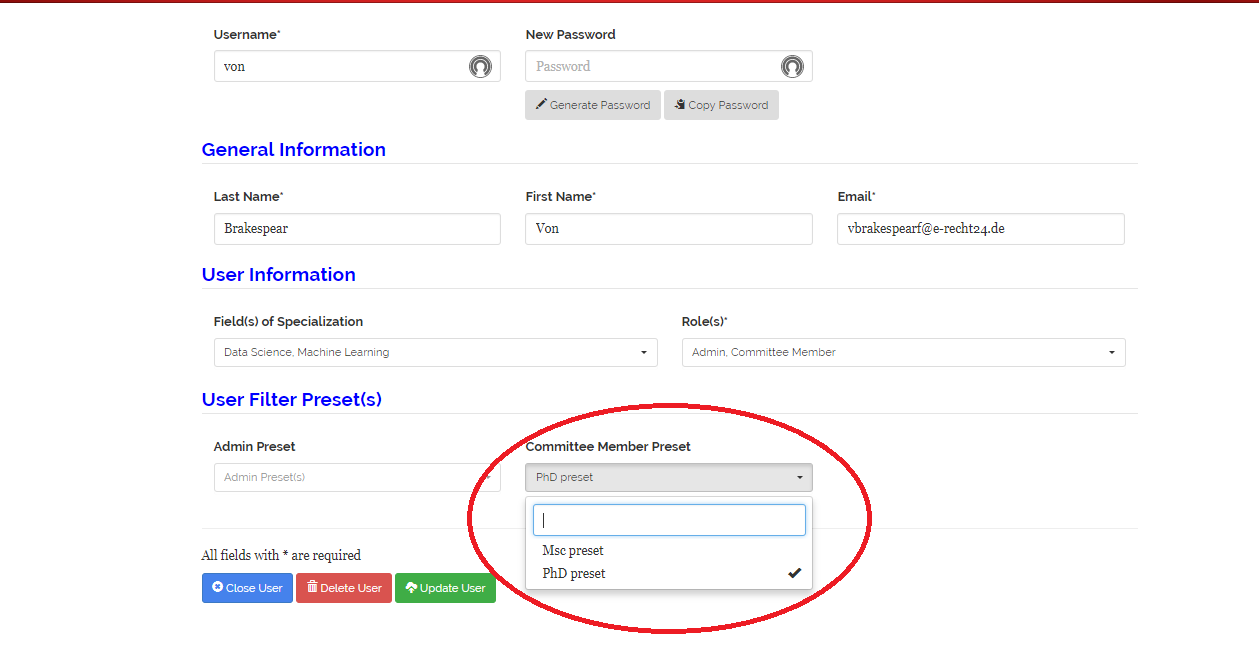
\includegraphics[width=.99\textwidth]{images/mu/remove_preset.png}
\end{center}
\caption{Remove Filter Presets}
\label{fig:remove_preset}
\end{figure}


\subsection{Sorting the Table}
If you wish to sort the table displayed simply click on the columns that display arrows next to the name. The table can be sorted in Ascending/Descending order described below.

\begin{itemize}
\item \textbf{Member Name:} Descending Order = Z to A, Ascending order = A to Z
\item \textbf{Member Email:} Descending Order = Z to A, Ascending order = A to Z
\end{itemize}

\textbf{Pro-tip:} To sort by multiple columns hold the shift key while clicking on the columns.

%%%%%%%%%%%% MANAGE APPLICATIONS %%%%%%%%%%%%

\newpage
\clearpage
\section{Manage Applications} \label{m_appls}
This section describes how you would create/delete an application, export applications to CSV, apply filtering on application(s), save most used filter(s) as preset and viewing application PDF file. To begin, from the administrator dashboard, click on \emph{Manage Applications}.

\begin{figure}[!htb]
\begin{center}
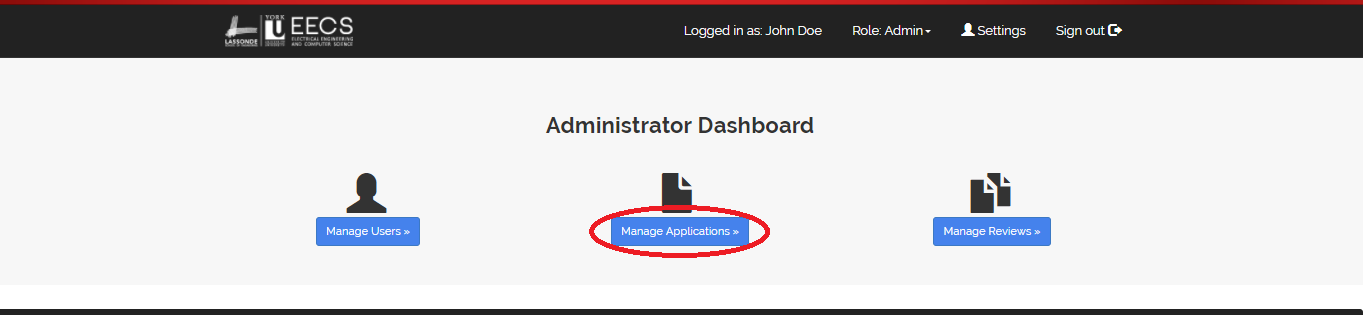
\includegraphics[width=.99\textwidth]{images/ma/manage_app.png}
\end{center}
\caption{Click to Manage Applications}
\label{fig:manage_app}
\end{figure}

\subsection{Create an application} \label{c_appl}
Once in the managing application portal, you can create a new application and upload all necessary documents. Creating a new application requires you to upload the application file, filling out general application information, previous grades, application information and finally assigning a one or more reviewer from the admission graduate committee. The following fields are required when creating a new application:
\begin{itemize}
\item Application File
\item Session
\item Student Number
\item Last Name
\item First Name
\item Email
\item Gender
\item GPA
\item Visa Status
\item Degree Applied For
\item Field(s) of Interest
\item Preferred Professor(s)
\end{itemize}

\begin{figure}[!htb]
\begin{center}
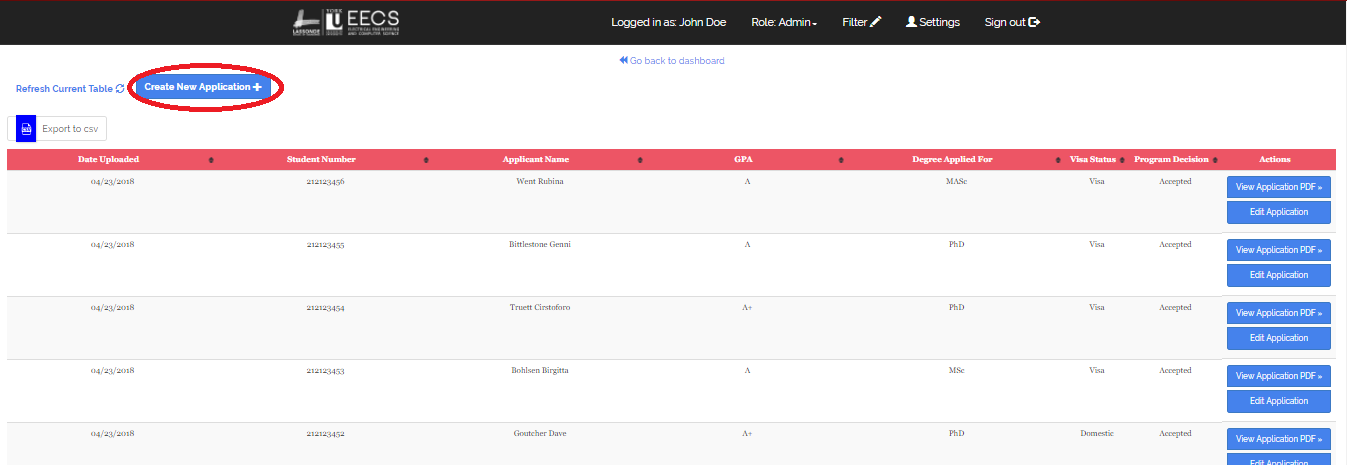
\includegraphics[width=.99\textwidth]{images/ma/new_app_click.png}
\end{center}
\caption{Click to create a application}
\label{fig:new_app_click}
\end{figure}

\clearpage
\begin{figure}[!htb]
\begin{center}
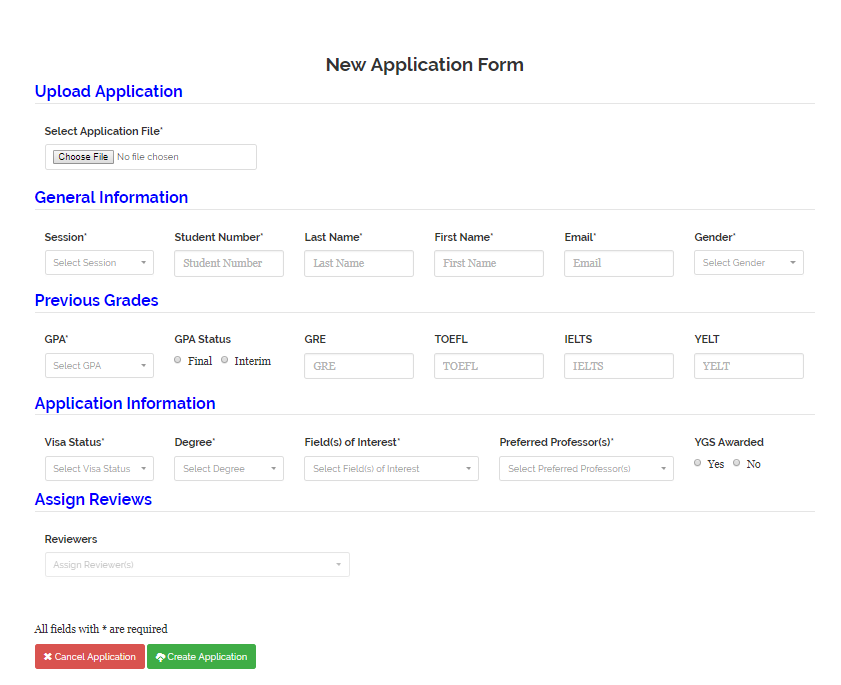
\includegraphics[width=.99\textwidth]{images/ma/fill_in_app.png}
\end{center}
\caption{Filling in application}
\label{fig:fill_in_app}
\end{figure}

\smallskip
\noindent \textbf{Note:} The maximum application file size for upload is set to 4MB and only accepted format of file accepted is PDF.

\clearpage
\subsection{Edit existing application}
Once in the managing application portal, you can edit an existing application. Editing includes updating all attributes specified in the previous section (refer to Section \ref{c_appl}) plus additional attributes such as professor(s) that have contacted or requested the student, the program decision, the student decision and etc.

\begin{figure}[!htb]
\begin{center}
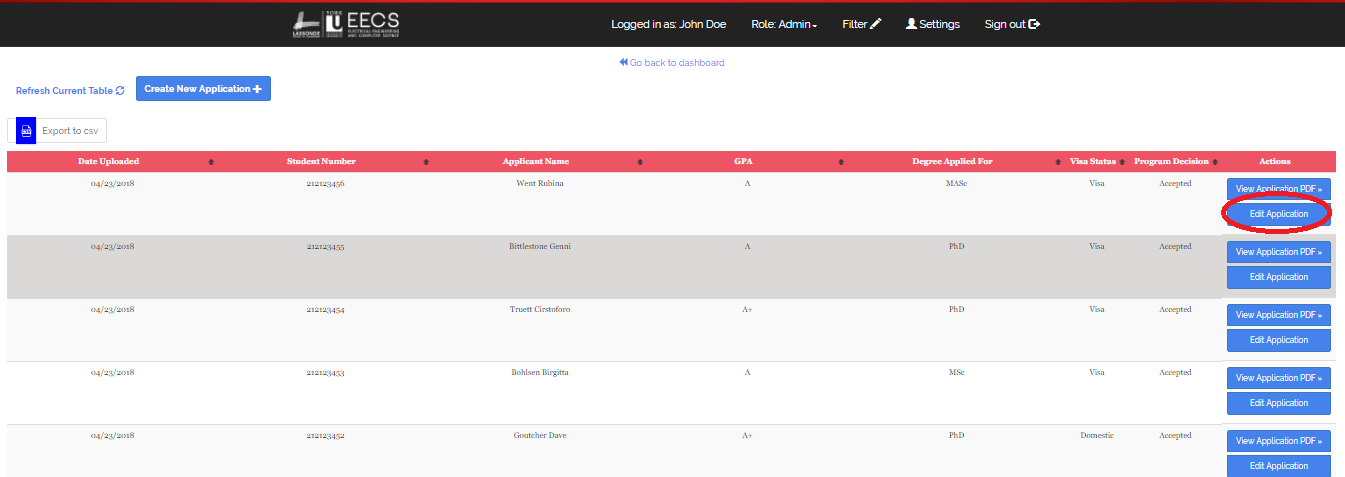
\includegraphics[width=.99\textwidth]{images/ma/edit_appl.png}
\end{center}
\caption{Click to edit an application}
\label{fig:edit_appl}
\end{figure}

\clearpage
\subsubsection{Remove an application}
To remove an existing application from the system, click on the \emph{Manage Applications} button as shown above for the corresponding application. Then click on the trash can button at the bottom of the page as shown.

\begin{figure}[!htb]
\begin{center}
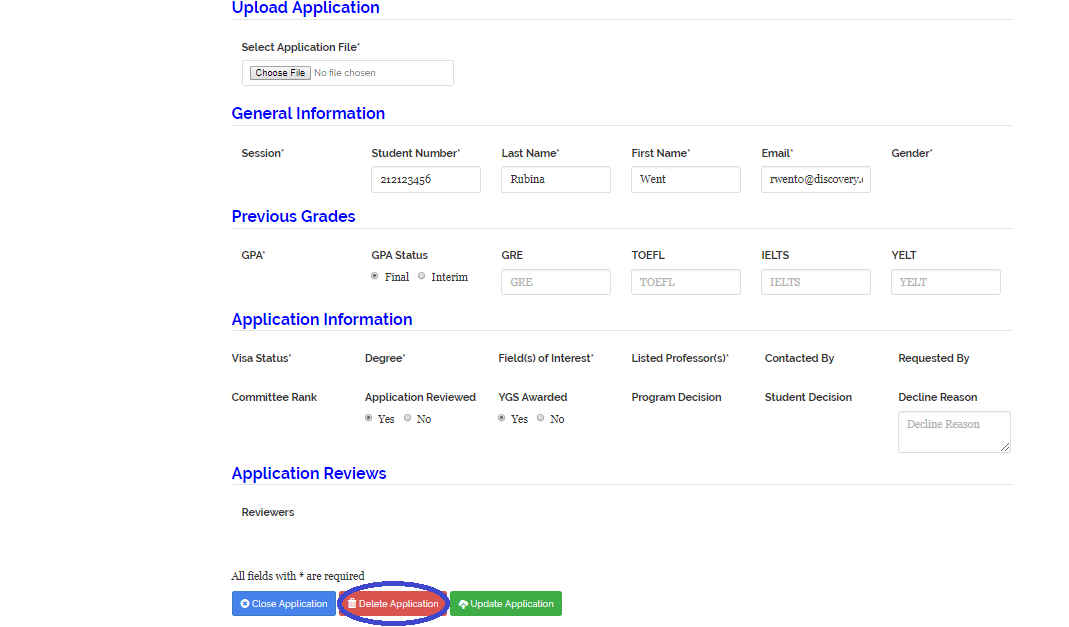
\includegraphics[width=.99\textwidth]{images/ma/remove_appl.png}
\end{center}
\caption{Removing an application}
\label{fig:remove_appl}
\end{figure}

\clearpage
\subsubsection{Update an application}
To update an existing application from the system, click on the \emph{Manage Applications} button as shown above for the corresponding application. Then click on the upload button at the bottom of the page as shown. The fields that are required when editing an application is the same as when creating an application.

\begin{figure}[!htb]
\begin{center}
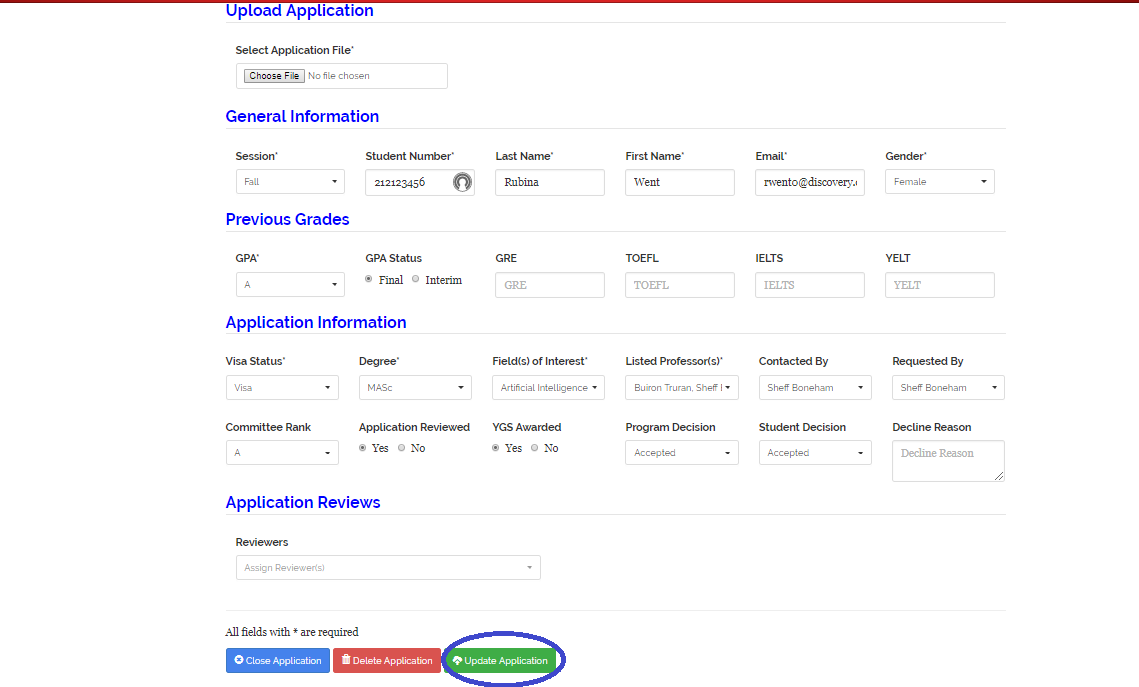
\includegraphics[width=.99\textwidth]{images/ma/update_appl.png}
\end{center}
\caption{Updating an application}
\label{fig:update_appl}
\end{figure}

\clearpage
\subsection{Export Application(s)}
Once in the managing application portal, you export all or a set of application(s) in CSV format. To achieve a set of applications simply use filtering to narrow down the application result. Clicking on the \emph{Export to CSV} button will download all selected application into a CSV file.

\begin{figure}[!htb]
\begin{center}
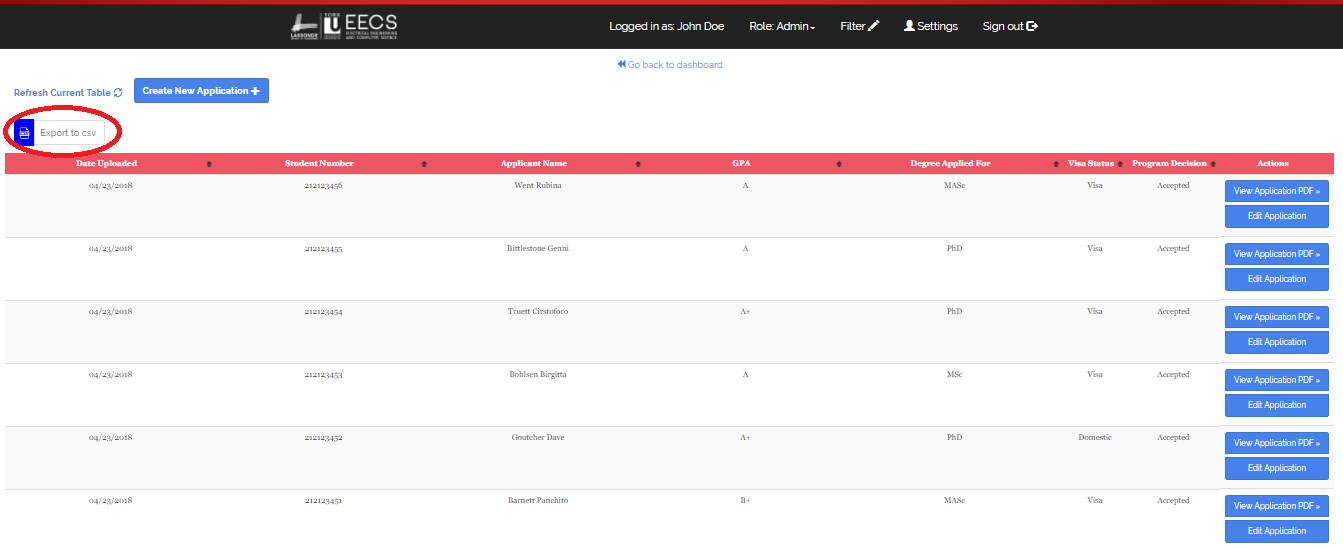
\includegraphics[width=.99\textwidth]{images/ma/export_appl.png}
\end{center}
\caption{Exporting application(s)}
\label{fig:export_appl}
\end{figure}

\clearpage
\subsection{View Application PDF}
Once in the managing application portal, you can chose to view the PDF formatted file of the application. Clicking on the \emph{View Application PDF} for the corresponding application will open a new tab along with the pdf file.

\begin{figure}[!htb]
\begin{center}
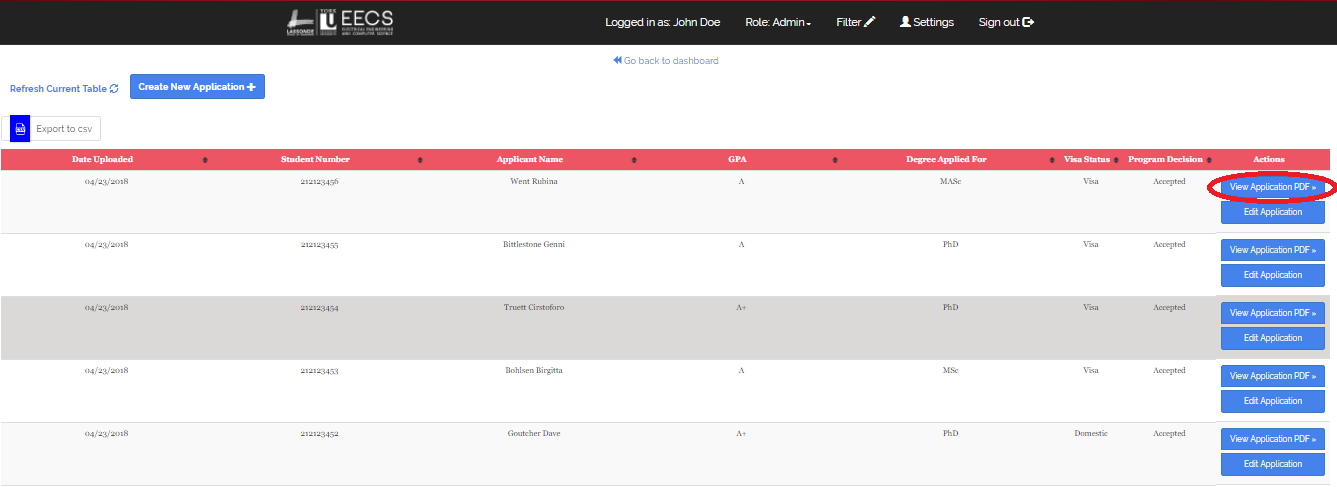
\includegraphics[width=.9\textwidth]{images/ma/view_appl_app.png}
\end{center}
\caption{Viewing Application PDF}
\label{fig:view_appl_app}
\end{figure}

\begin{figure}[!htb]
\begin{center}
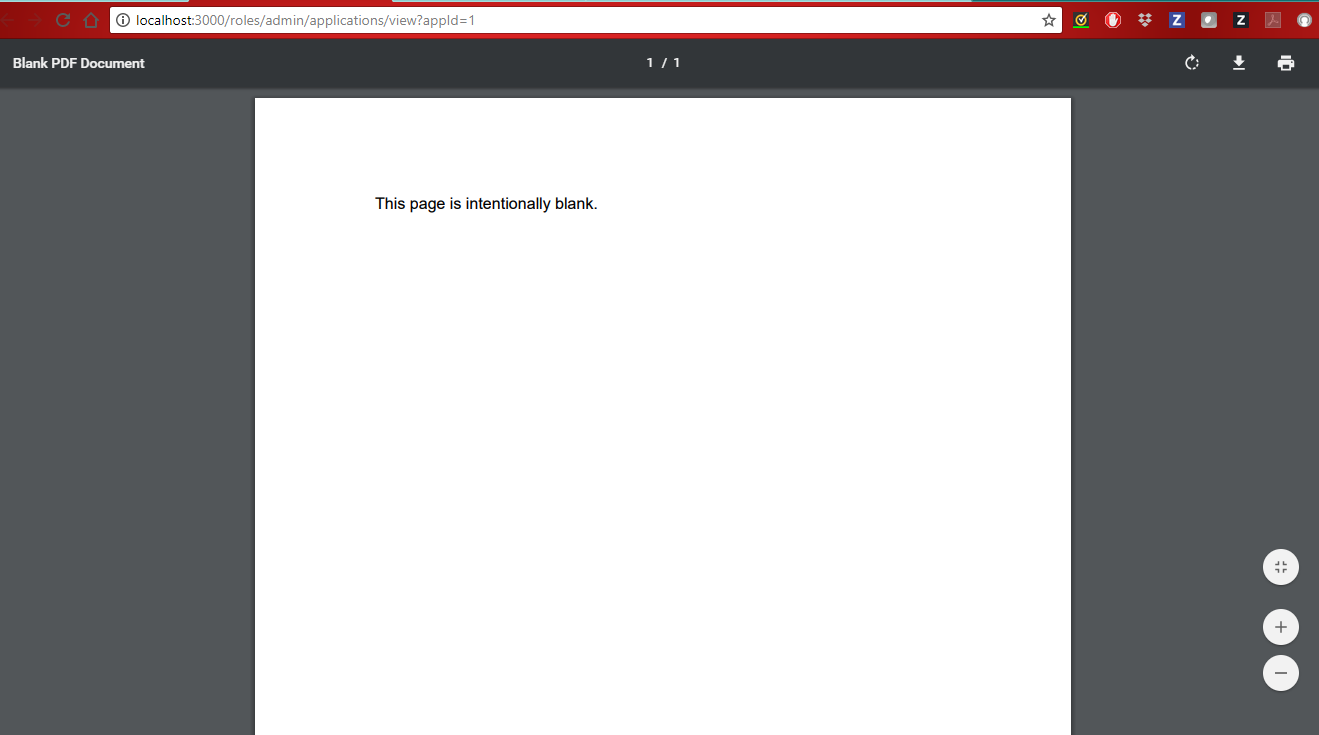
\includegraphics[width=.9\textwidth]{images/ma/appl_pdf.png}
\end{center}
\caption{Application PDF}
\label{fig:appl_pdf}
\end{figure}

\clearpage
\subsection{Filtering the Table}
This section describes how you would use/build/save/load a filter on the review table.

\subsubsection{Opening the Modal}
To begin with filtering you must open the modal. To do so click on the ``Filter" button on the navigation bar.

\begin{figure}[!htb]
\begin{center}
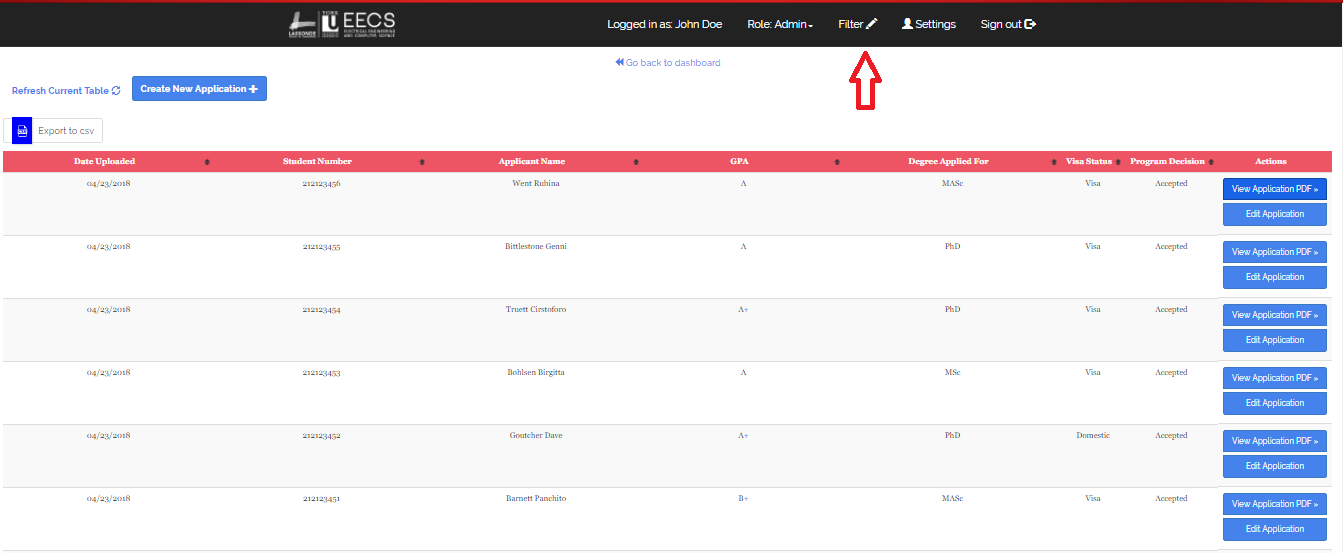
\includegraphics[width=.99\textwidth]{images/ma/open_modal.png}
\end{center}
\caption{Opening the  Modal}
\label{fig:open_modal}
\end{figure}

\begin{figure}[!htb]
\begin{center}
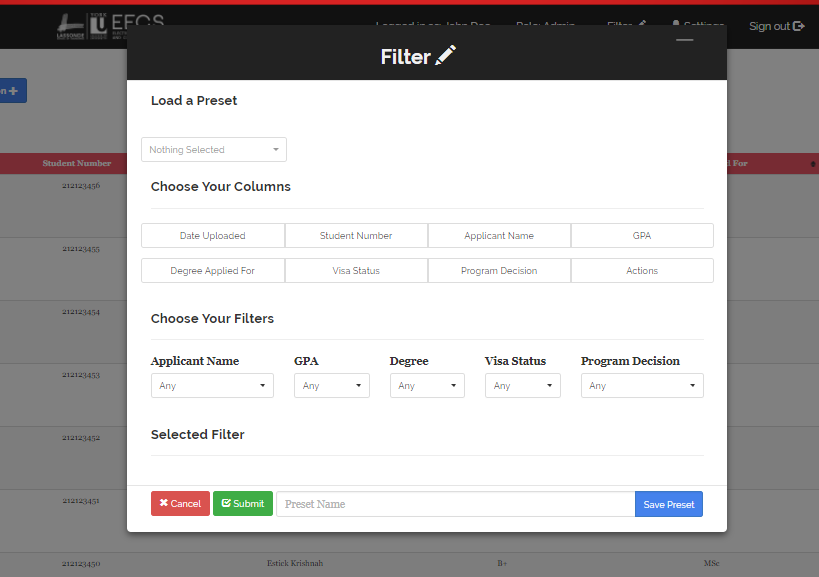
\includegraphics[width=.99\textwidth]{images/ma/default_filter_view.png}
\end{center}
\caption{Filter View}
\label{fig:filter_view}
\end{figure}

\clearpage
\newpage

\begin{figure}[!htb]
\subsubsection{Choose Your Columns}
Once the modal is opened you can then choose the columns you wish to be displayed on the table. To do so, click on the button indicating which column you wish to see. Once clicked the button will display the order that column will appear in the table.

\begin{center}
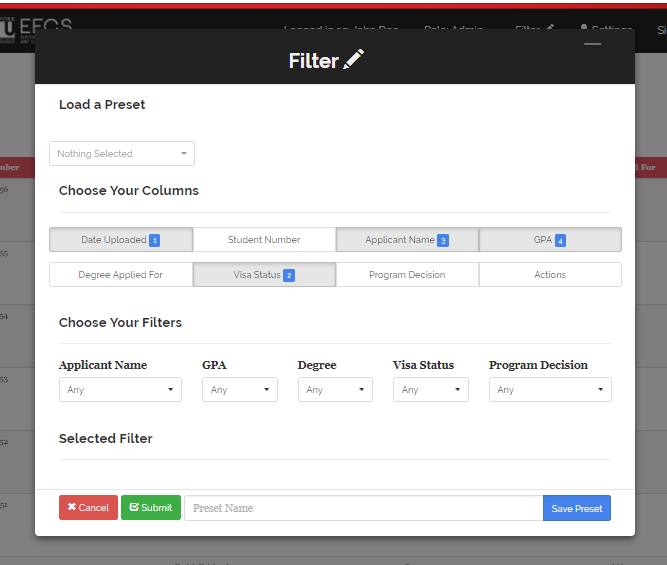
\includegraphics[width=.99\textwidth]{images/ma/selected_col.png}
\end{center}
\caption{Choose Your Columns}
\label{fig:choose_columns}

\smallskip
\noindent \textbf{Note:} Not selecting any column will use the same columns and order as the default table. If the \emph{Actions} column is not selected it will automatically be placed as the right most column. 
\end{figure}

\clearpage
\begin{figure}[!htb]
\subsubsection{Choose Your Filters}
After selecting your columns, you can then choose the attributes by which you wish to filter your table. Begin by clicking on the drop down of the attribute you wish to filter and select an option from a list of generated options.

\begin{center}
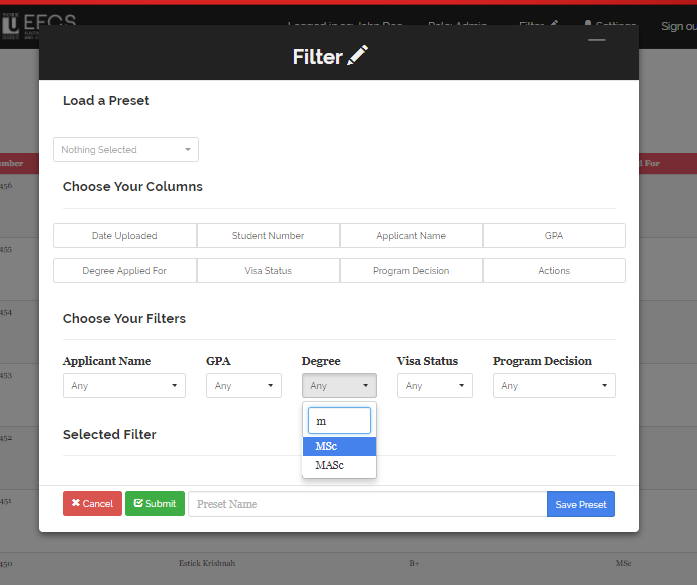
\includegraphics[width=.99\textwidth]{images/ma/selected_filter.png}
\end{center}
\caption{Choose Your Filters}

\smallskip
\noindent \textbf{Note:} You can use the search bar to help locate values. Begin by typing in the text box displayed. You can only select an option that appears in the dropdown.
\label{fig:choose_filters}
\end{figure} 

\clearpage 
\begin{figure}[!htb]
\subsubsection{Submitting a Filter}
Once you have chosen your columns and filter attributes confirm your filter by reading the text under ``Selected Filter'' and click ``Submit". The text under the ``Selected Filter'' will change based on your filter attributes.

\begin{center}
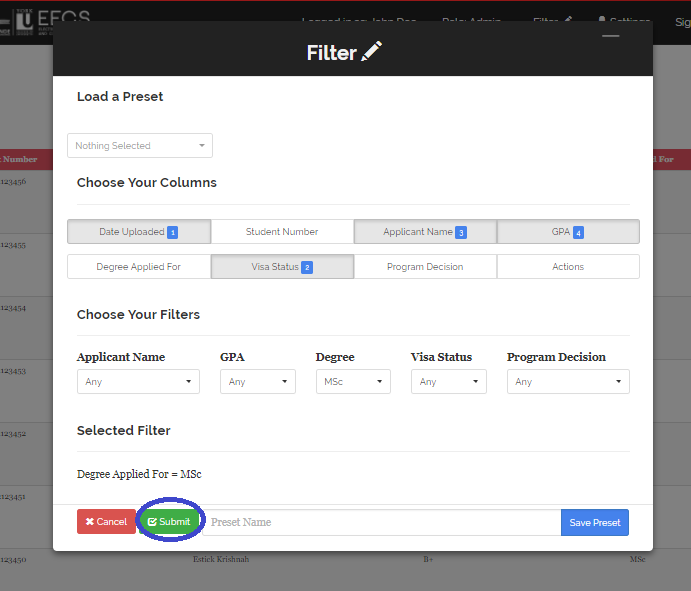
\includegraphics[width=.99\textwidth]{images/ma/submit_filter.png}
\end{center}
\caption{Submit Filter}
\textbf{Note}: When submitting a filter with no selected filters, the default table will be loaded.
\label{fig:submit_filter}
\end{figure}

\begin{figure}[!htb]
\begin{center}
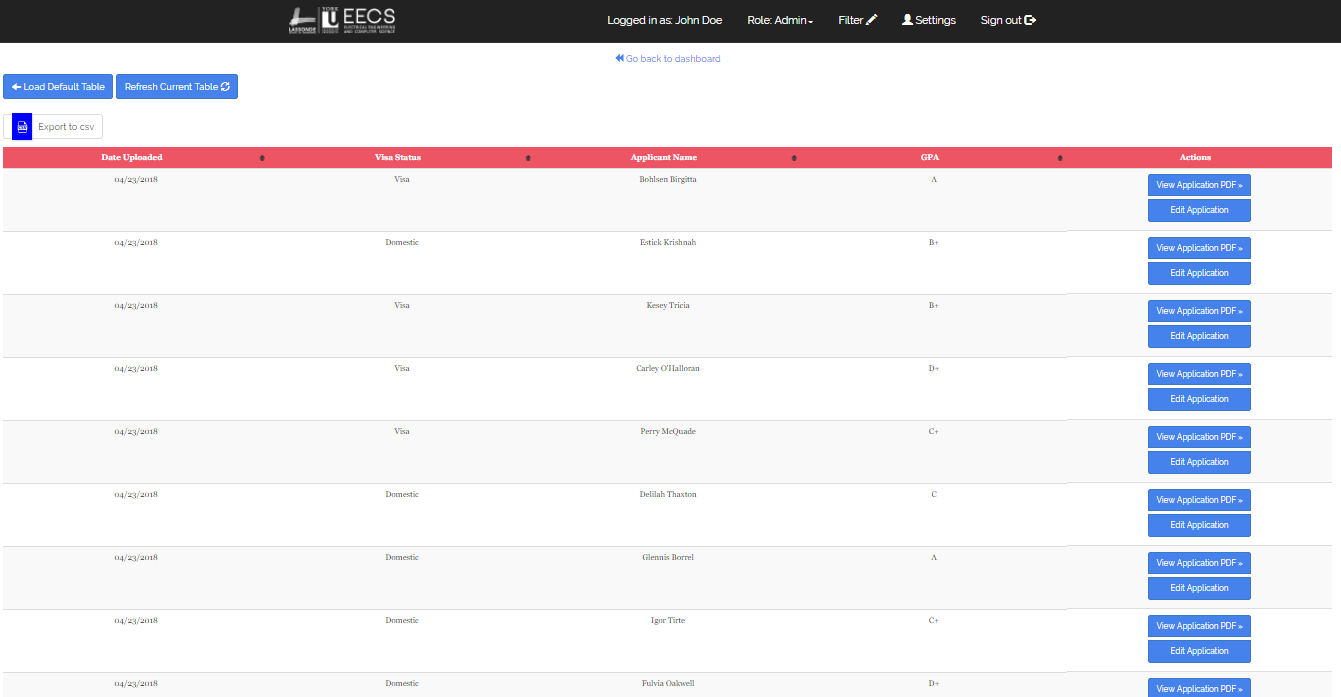
\includegraphics[width=.99\textwidth]{images/ma/example_filter_table.png}
\end{center}
\caption{Resulted Table After Applying Filter}
\label{fig:resulted_table}
\end{figure}

\clearpage

\begin{figure}[!htb]
\subsubsection{Saving a Filter}
Once you have chosen your columns and filter attributes confirm your filter by reading the text under ``Selected Filter'' and give the preset a name by typing in the text box between the ``Submit'' and the ``Save Preset'' button. Once that is done click ``Save Preset''.

\begin{center}
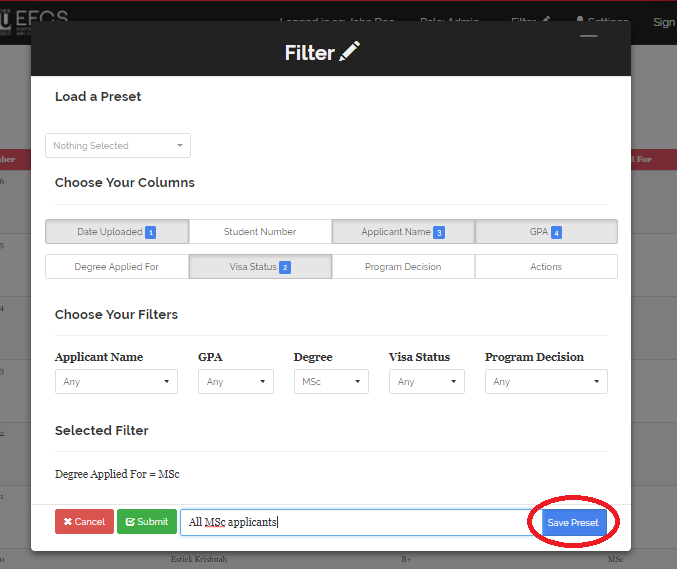
\includegraphics[width=.99\textwidth]{images/ma/saving_preset.png}
\end{center}
\caption{Save a Filter}
\label{fig:save_filter}
\end{figure}

\smallskip
\noindent Once you have saved a filter you will be provided with a new table to match your filter and it will appear in the dropdown to be used for loading a filter.

\smallskip
\noindent \textbf{Pro-tip:} You can update a filter by typing in the same name as an existing filter.

\clearpage
\begin{figure}[!htb]
\subsubsection{Loading a Filter}
To load a saved filter click the dropdown under ``Load a Preset'' and select the preset you wish to use. Once selected the modal will auto-populate.

\begin{center}
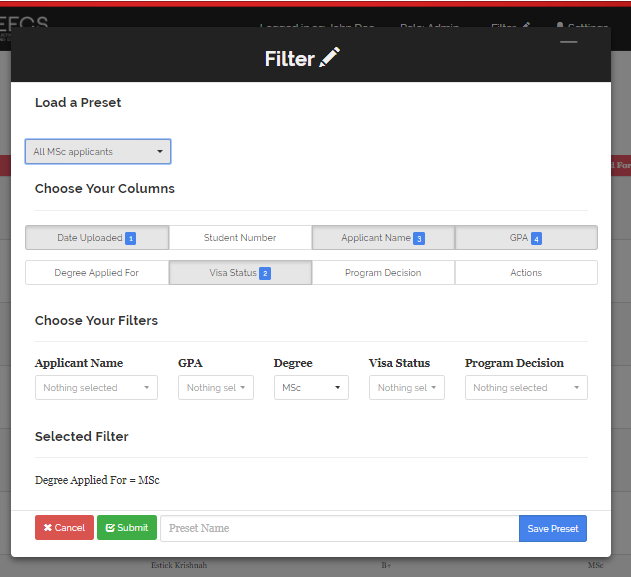
\includegraphics[width=.99\textwidth]{images/ma/load_preset.png}
\end{center}
\caption{Loading a Filter}
\label{fig:save_filter}
\end{figure}

\smallskip
\noindent \textbf{Pro-tip:} Create a preset called \emph{Default} with no columns or filters selected. You can then use this to load the default table or help clear any data you put in the modal.

\clearpage
\subsection{Sorting the Table}
If you wish to sort the table displayed simply click on the columns that display arrows next to the name. The table can be sorted in Ascending/Descending order described below.
\begin{itemize}
\item \textbf{Date Uploaded:} Descending Order = Newest - Oldest, Ascending order = Oldest - Newest
\item \textbf{Student Number:} Descending Order = Largest to Smallest, Ascending order = Smallest to Largest
\item \textbf{Applicant Name:} Descending Order = Z to A, Ascending order = A to Z
\item \textbf{GPA:} Descending Order = A+ to F, Ascending order = F to A+
\item \textbf{Degree Applied For:} Descending Order = Z to A, Ascending order = A to Z
\item \textbf{Program Decision:} Descending Order = Z to A, Ascending order = A to Z
\end{itemize}
\textbf{Pro-tip:} To sort by multiple columns hold the shift key while clicking on the columns.

\bigskip
\noindent \textbf{Note}: Ordering fields can be done on both filtered and unfiltered application lists.

\bigskip
\noindent The following images depicts on how to order review applications using the \emph{Student Number} field in ascending and descending order.

\begin{figure}[!htb]
\begin{center}
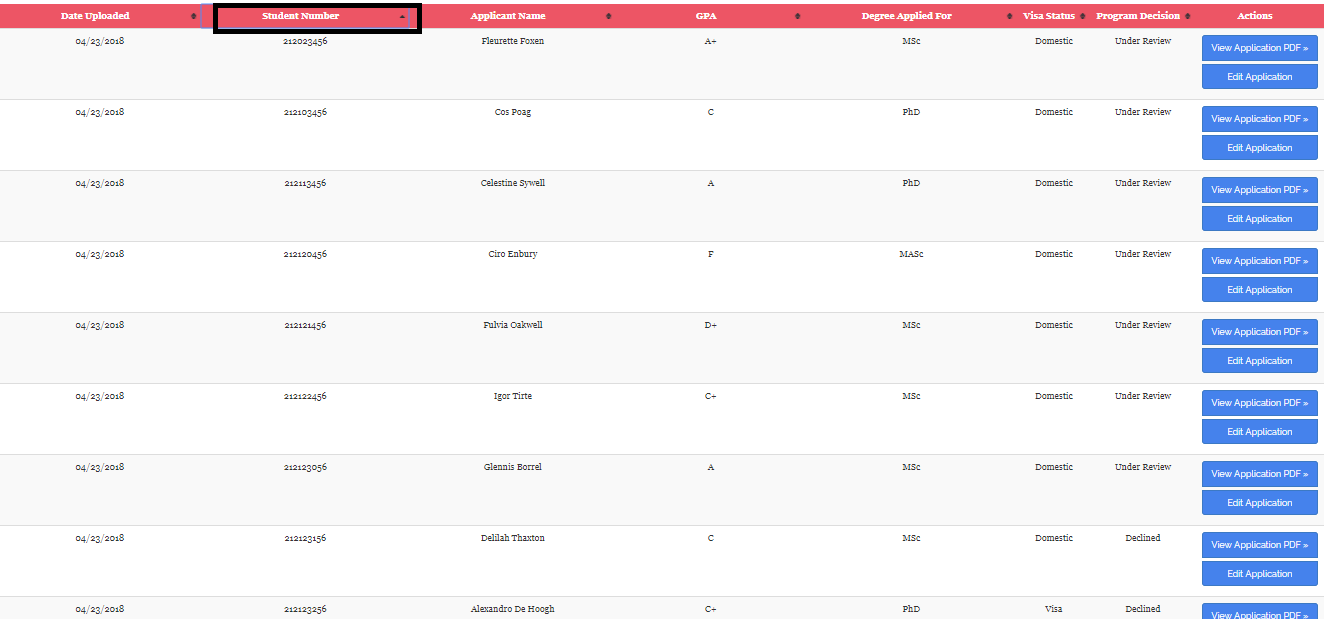
\includegraphics[width=.99\textwidth]{images/ma/order_ascending.png}
\end{center}
\caption{Ascending order of Student Number field}
\label{fig:order_ascending}
\end{figure}

\begin{figure}[!htb]
\begin{center}
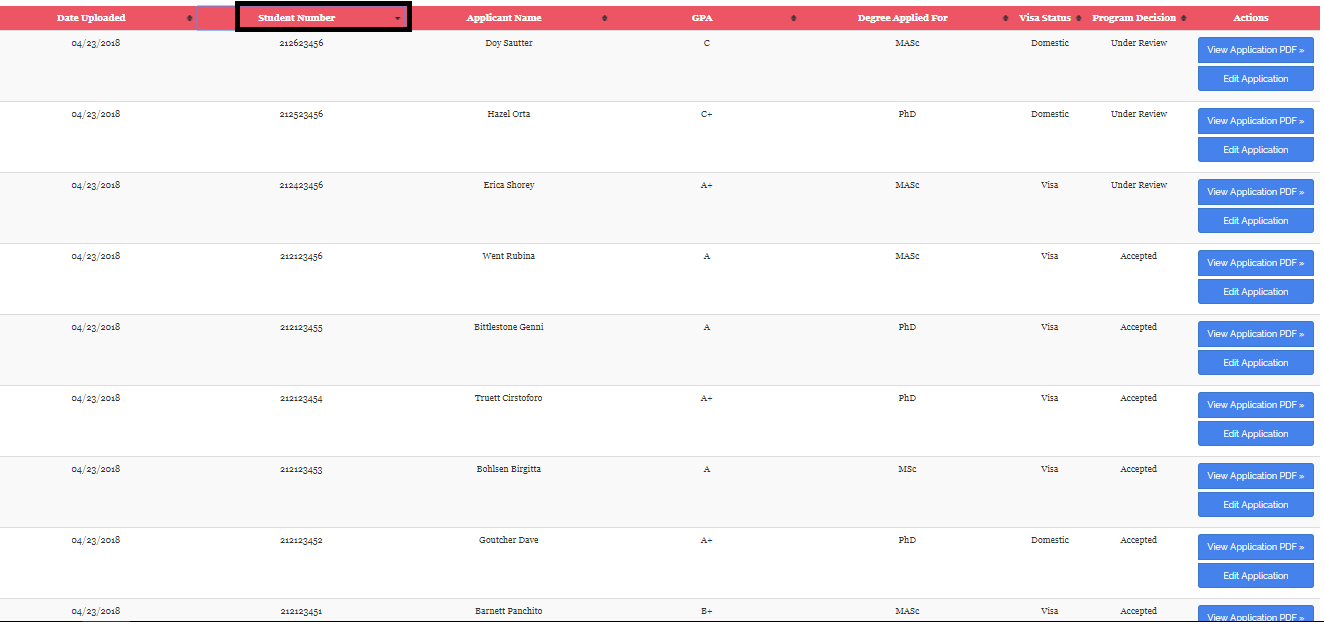
\includegraphics[width=.99\textwidth]{images/ma/order_descending.png}
\end{center}
\caption{Descending order of Student Number field}
\label{fig:order_descending}
\end{figure}

\newpage

\begin{figure}[!htb]
\begin{center}
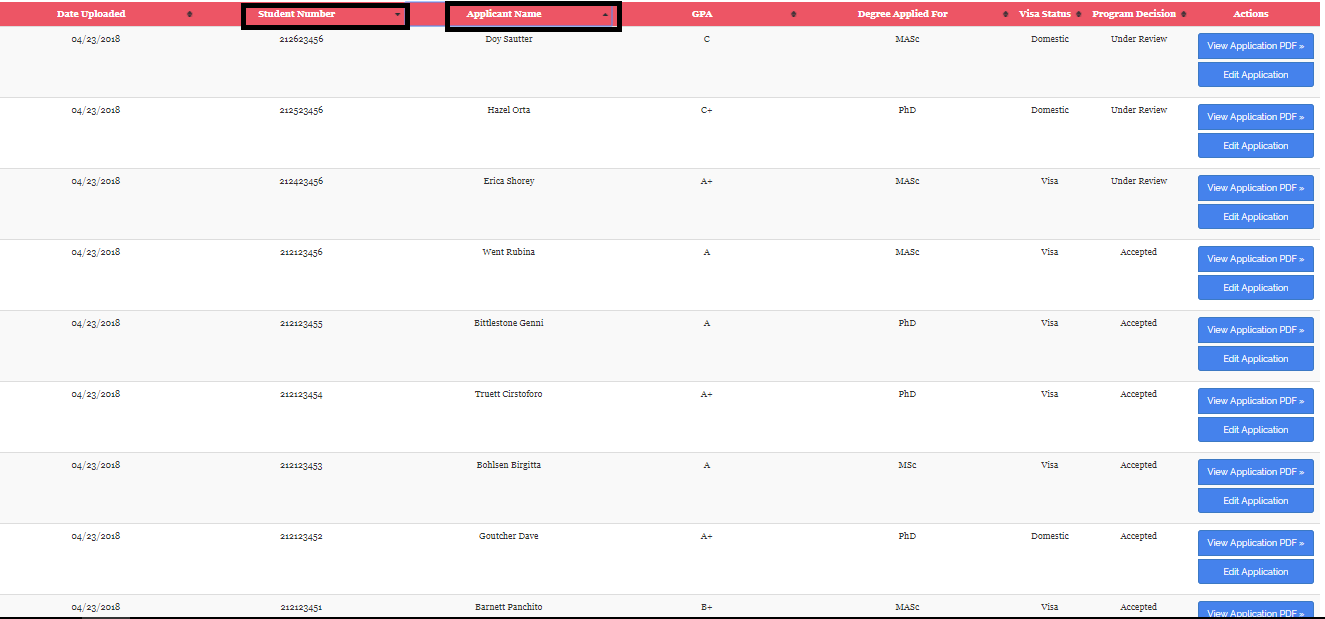
\includegraphics[width=.99\textwidth]{images/ma/multiple_order.png}
\end{center}
\caption{Ordering using multiple fields}
\label{fig:multiple_order}
\end{figure}

%%%%%%%%%%%% MANAGE REVIEWS %%%%%%%%%%%%

\newpage
\clearpage
\section{Manage Reviews} \label{m_reviews}
This section describes how you would assign, unassign or dismiss reviews for an application and apply filter on review applications. To begin, from the administrator dashboard, click on \emph{Manage Reviews}.

\begin{figure}[!htb]
\begin{center}
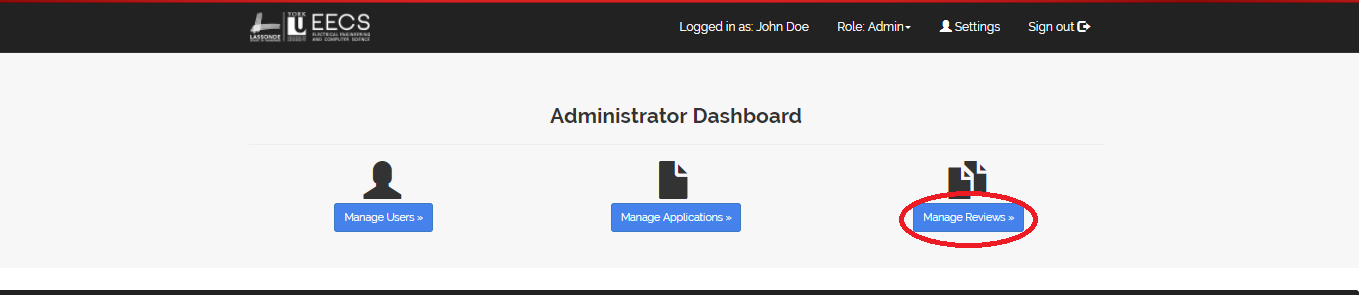
\includegraphics[width=.99\textwidth]{images/mr/manage_review.png}
\end{center}
\caption{Click to Manage Reviews}
\label{fig:manage_review}
\end{figure}


\subsection{Assign Review}
Once in the managing review portal, you can assign a reviewer to an application. There is a maximum cap of number of reviewers assigned to an application. For domestic applications there is a maximum of 2 reviewers whereas for visa applications there is a maximum of 1 reviewer.

\begin{figure}[!htb]
\begin{center}
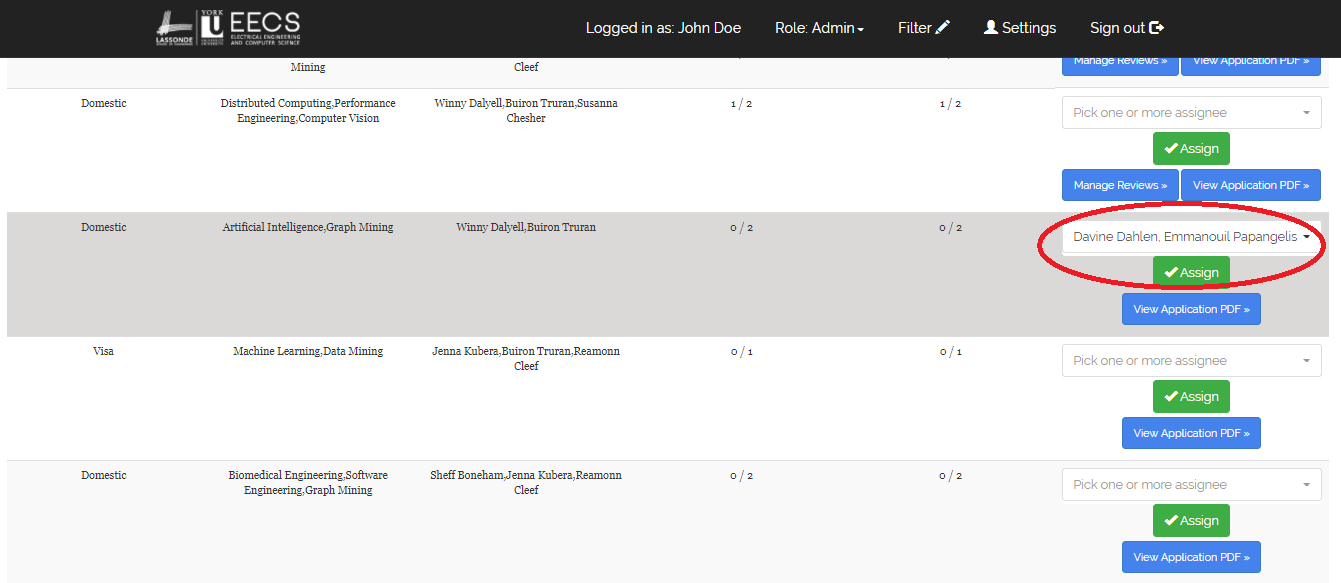
\includegraphics[width=.99\textwidth]{images/mr/assign_review.png}
\end{center}
\caption{Assign a review}
\label{fig:assign_review}
\end{figure}

\subsection{Unassign Review}
Once in the managing review portal, you can manage a review for the corresponding application. To manage the review, click on \emph{Manage Reviews} for the corresponding application. In the review outline page, it will display all the reviewers for the application. You can unassign a review for an application if it has not been submitted yet.

\begin{figure}[!htb]
\begin{center}
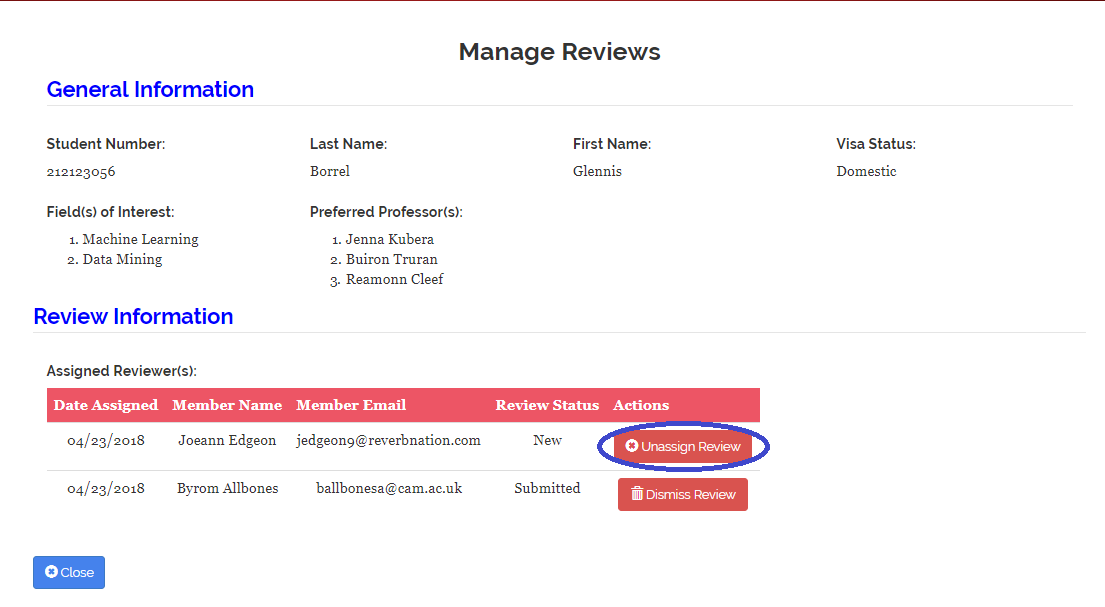
\includegraphics[width=.99\textwidth]{images/mr/unassign_review.png}
\end{center}
\caption{Unassign a review}
\label{fig:unassign_review}
\end{figure}

\clearpage
\subsection{Dismiss Review}
Once in the managing review portal, you can manage a review for the corresponding application. To manage the review, click on \emph{Manage Reviews} for the corresponding application. In the review outline page, it will display all the reviewers for the application. You can dismiss a review for an application if it has been already submitted.

\begin{figure}[!htb]
\begin{center}
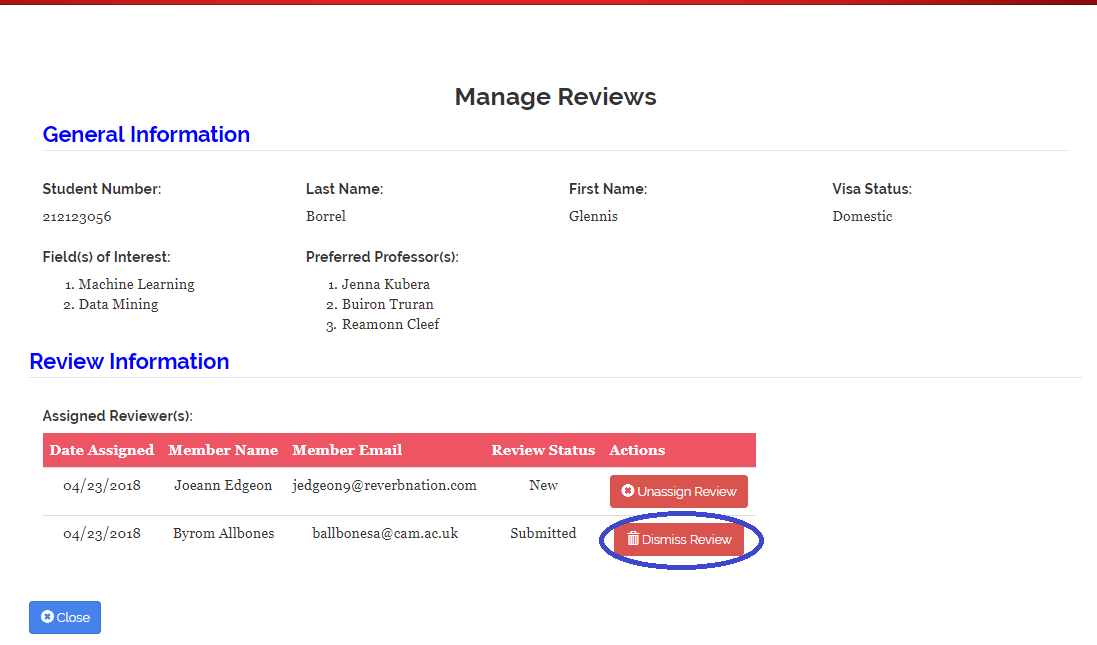
\includegraphics[width=.99\textwidth]{images/mr/dismiss_review.png}
\end{center}
\caption{Dismiss a review}
\label{fig:dismiss_review}
\end{figure}

\clearpage
\subsection{Filtering the Table}
This section describes how you would use/build a filter on the table.

\subsubsection{Opening the Modal}
To begin with filtering you must open the modal. To do so click on the ``Filter" button on the navigation bar.

\begin{figure}[!htb]
\begin{center}
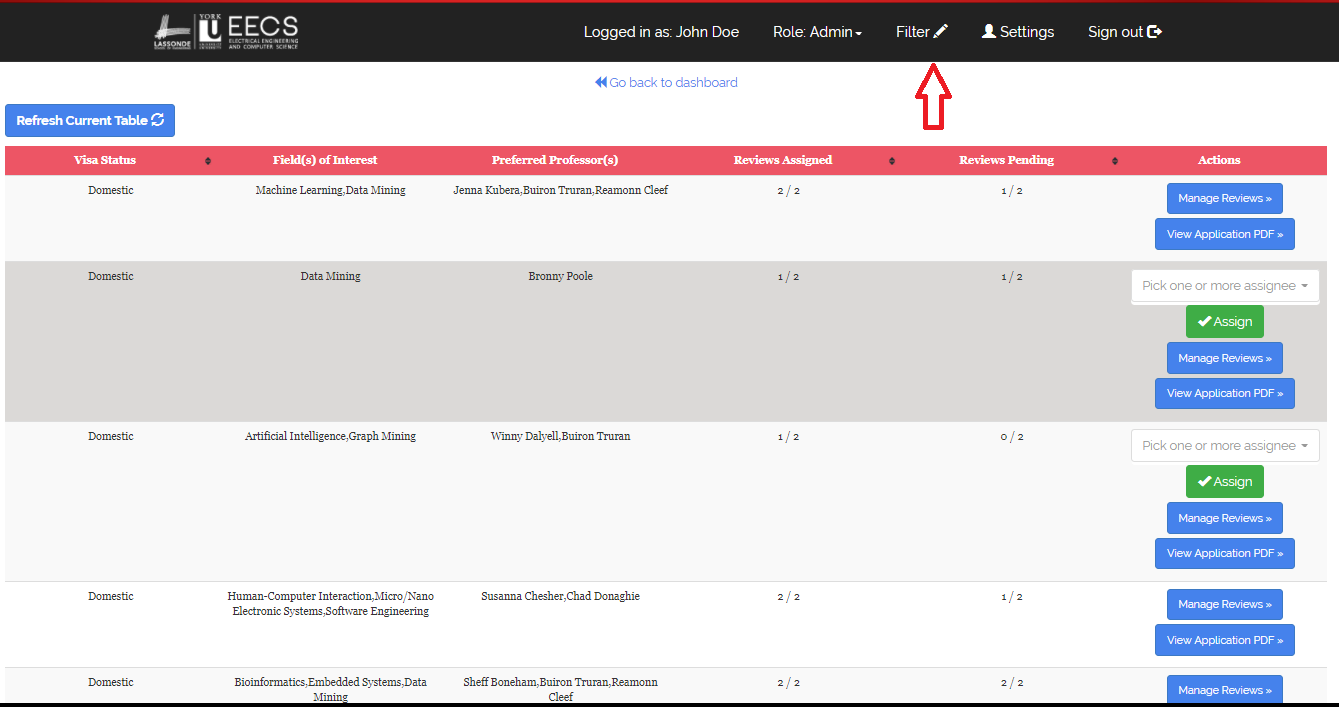
\includegraphics[width=.99\textwidth]{images/mr/open_modal.png}
\end{center}
\caption{Opening the  Modal}
\label{fig:open_modal}
\end{figure}

\clearpage
\newpage

\begin{figure}[!htb]
\subsubsection{Choose Your Columns}
Once the modal is opened you can then choose the columns you wish to be displayed on the table. To do so, click on the button indicating which column you wish to see. Once clicked the button will display the order that column will appear in the table.

\begin{center}
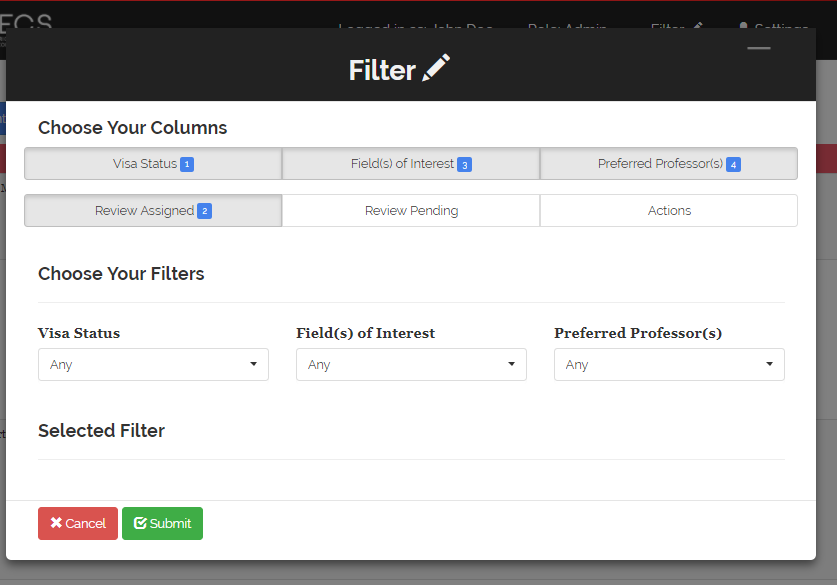
\includegraphics[width=.99\textwidth]{images/mr/selected_col.png}
\end{center}
\caption{Choose Your Columns}
\label{fig:choose_columns}

\smallskip
\noindent \textbf{Note:} Not selecting any column will use the same columns and order as the default table. If the \emph{Actions} column is not selected it will automatically be placed as the right most column. 
\end{figure}

\clearpage
\begin{figure}[!htb]
\subsubsection{Choose Your Filters}
After selecting your columns, you can then choose the attributes by which you wish to filter your table. Begin by clicking on the drop down of the attribute you wish to filter and select an option from a list of generated options.

\begin{center}
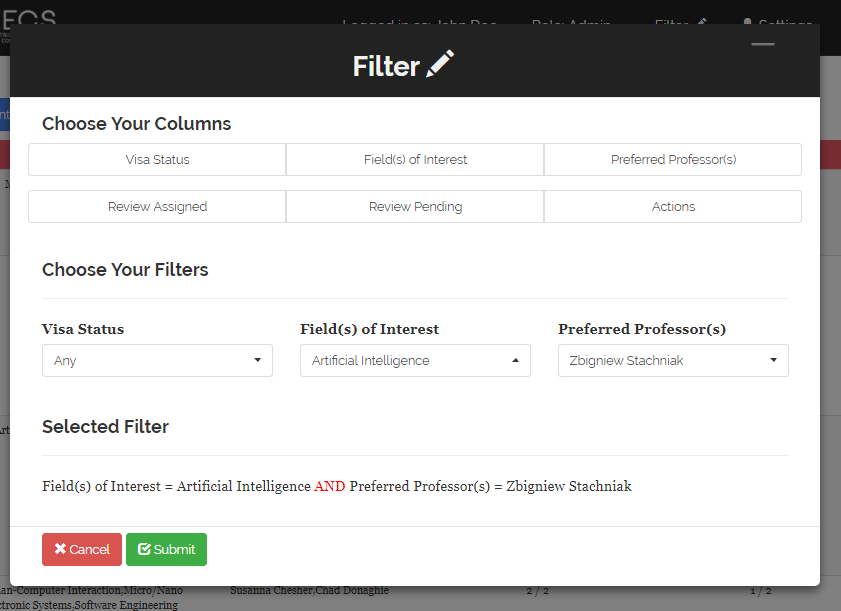
\includegraphics[width=.99\textwidth]{images/mr/selected_filter.png}
\end{center}
\caption{Choose Your Filters}

\smallskip
\noindent \textbf{Note:} You can use the search bar to help locate values. Begin by typing in the text box displayed. You can only select an option that appears in the dropdown.
\label{fig:choose_filters}
\end{figure} 

\clearpage 
\begin{figure}[!htb]
\subsubsection{Submitting a Filter}
Once you have chosen your columns and filter attributes confirm your filter by reading the text under ``Selected Filter'' and click ``Submit". The text under the ``Selected Filter'' will change based on your filter attributes.

\bigskip
\noindent Once a resulted set of table is returned after filtering, you can assign/unassign/dismiss review from any of the returned applications.

\begin{center}
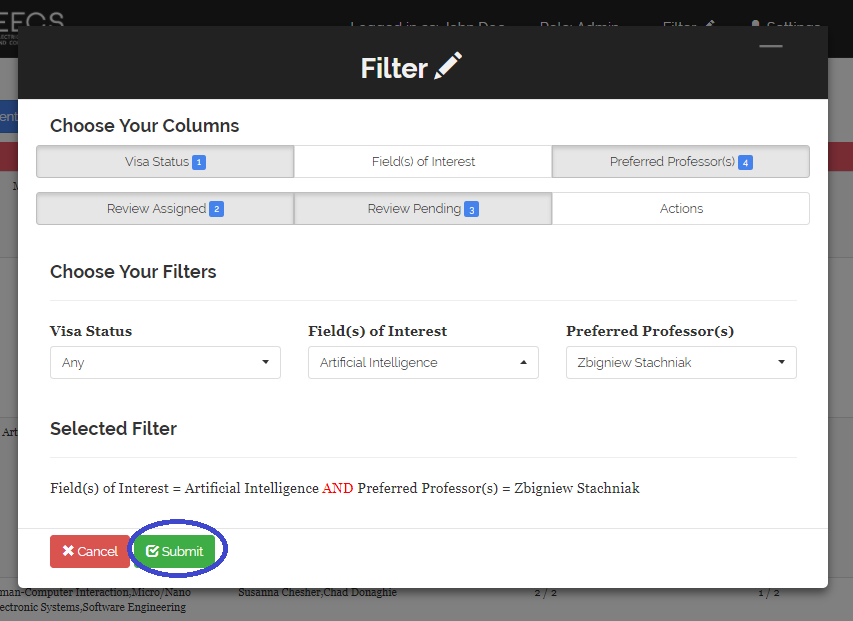
\includegraphics[width=.99\textwidth]{images/mr/submit_filter.png}
\end{center}
\caption{Submit Filter}
\textbf{Note}: When submitting a filter with no selected filters, the default table will be loaded.
\label{fig:submit_filter}
\end{figure}

\begin{figure}[!htb]
\begin{center}
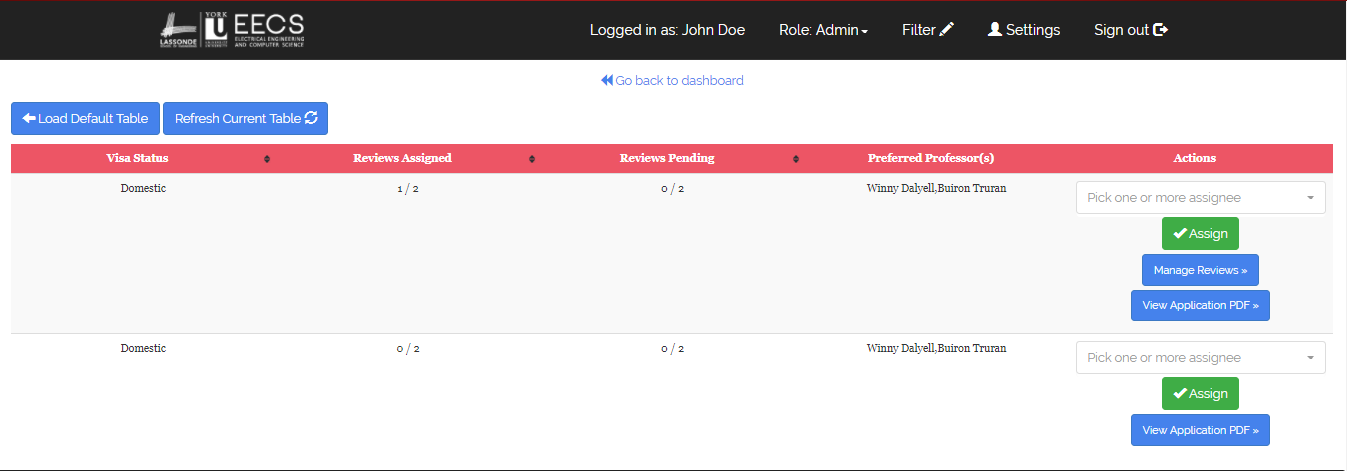
\includegraphics[width=.99\textwidth]{images/mr/example_filter_table.png}
\end{center}
\caption{Resulted Table After Applying Filter}
\label{fig:resulted_table}
\end{figure}

\subsection{Sorting the Table}
If you wish to sort the table displayed simply click on the columns that display arrows next to the name. The table can be sorted in Ascending/Descending order described below.
\begin{itemize}
\item \textbf{Visa Status:} Descending Order = Z to A, Ascending order = A to Z
\item \textbf{Review Assigned:} Descending Order = Largest to Smallest, Ascending order = Smallest to Largest
\item \textbf{Review Pending:} Descending Order = Largest to Smallest, Ascending order = Smallest to Largest
\end{itemize}
\textbf{Pro-tip:} To sort by multiple columns hold the shift key while clicking on the columns.

\bigskip
\noindent \textbf{Note}: Ordering fields can be done on both filtered and unfiltered review application lists.

\end{document}